\documentclass[12pt]{article}

% PACOTES

% Tipografia

\usepackage[utf8]{inputenc}
\usepackage{xcolor}
\usepackage{amsfonts, amsmath, amssymb}

%\usepackage{arev}
%\usepackage[T1]{fontenc}
%\usepackage[math]{iwona}
%\usepackage[T1]{fontenc}
%\usepackage[scaled]{helvet}
%\renewcommand\familydefault{\sfdefault} 
%\usepackage[T1]{fontenc}
\usepackage{sansmathfonts}
\usepackage[T1]{fontenc}
\renewcommand*\familydefault{\sfdefault}

% Layout

\usepackage[pagecolor={yellow!30}]{pagecolor}
\usepackage{geometry}
\geometry{paper=a4paper}
\geometry{top=3cm, left=3cm, bottom=2cm, right=2cm}

\usepackage{graphicx}
\usepackage[nottoc, notlot, notlof]{tocbibind}
\usepackage{float}
\usepackage{pbox}
\usepackage{enumitem}
\usepackage{tikz}
\usepackage{pgfplots}
\pgfplotsset{compat=1.5} 

\usepackage{array}
\renewcommand{\arraystretch}{1.5}
\newcolumntype{C}[1]{>{\centering\arraybackslash}p{#1}}

\usepackage{booktabs}
\usepackage{longtable}
\usepackage{tabularx}
\usepackage{multirow}
%\usepackage{fancyhdr}

%\graphicspath{{images/}}

\title{Formulário e Definições de Estatística}
\author{Daniel Vartanian}
\date{\today}

\parindent 0ex
\renewcommand{\baselinestretch}{1.5}
%\setlength{\parindent}{4em}
%\setlength{\parskip}{1em}
%\renewcommand{\headrulewidth}{0pt}
%\includeonly{}

\begin{document}

%\part{part}
%\chapter{chapter}
%\section{section}
%\subsection{subsection}
%\subsubsection{subsubsection}
%\paragraph{paragraph}
%\subparagraph{subparagraph}

	\begin{titlepage}

	\vfill
	\maketitle
	\vfill
	\thispagestyle{empty}
	\clearpage

\end{titlepage}

	\tableofcontents
\thispagestyle{empty}
\clearpage

	\setcounter{page}{1}

	\part{Estatística Descritiva}

	\section{Resumo de Dados}

	\section{Medidas Resumo}

	\subsection{Esquema dos 5 números}

	\subsection{Avaliação por medidas resumo}

	\subsection{Coeficientes de assimetria de Pearson}

	\subsection{Outros critérios}

	\subsection{Medidas de curtose}

	\subsection{Boxplot ou ``Caixa de Bigodes"}
	
	\section{Análise Bidimensional}
	
	\section{Análise Combinatória}

	\subsection{Princípios}

	\subsection{Permutações simples}

	\subsection{Arranjos}

	\subsection{Combinações}

	\clearpage

	\part{Probabilidades}

	\section{Probabilidades}

	\subsection{Propriedades básicas}

	\subsection{Diagrama em árvore}

	\subsection{Dependência/independência}

	\subsection{Teorema da Probabilidade Total}

	\subsection{Teorema de Bayes}

	\section{Variáveis Aleatórias Discretas}
	
	\section{Variáveis Aleatórias Contínuas}
	
	\section{Variáveis Aleatórias Multidimensionais}
	
	\section{Noções de Simulação}

	\clearpage

	\part{Inferência Estatística}

	\section{Introdução à Inferência Estatística}
	
	\section{Estimação}
	
	\section{Intervalos de Confiança}
	
	\section{Testes de Hipótese}
	
	\section{Inferência para Duas Populações}
	
	\section{Análise de Aderência e Associação}
	
	\section{Inferência para Várias Populações}
	
	\section{Regressão Linear}

Procedimentos Univariados

Teste K-S e Shapiro-Wilk

Análise de Outlier - Boxplot

Verificar os slides ``Introdução ao SPSS"

	\subsection{Método da Linha Reta}
	
		``É o tipo mais simples de ajustamento de curvas, cuja equação é
		
		\bigskip		
		
		{\Large $ Y = a + bX $} \ ,
		
		\bigskip
		
		onde  $ X $ e $ Y $ são variáveis e $ a $ e $ b $ são as constantes.

		Assim, dados dois pontos quaisquer $ (X1,Y1) $ e $ (X2,Y2) $ dessa reta, as constantes $ a $ e $ b $ podem ser determinadas" \cite{torres} .
	
		\subsubsection{Equação da Reta}
		
			``Podemos também considerar a forma mais comum de representar a função de 1º grau (função linear), ou seja, 
			
			\bigskip
			
			{\Large $ y = mx + n $} \ ;
			
			\bigskip
			
			onde $ b = m $ é coeficiente angular e $a = n$ é o coeficiente linear" . \cite{morettin}
			
			\bigskip			
			
			{\Large $ m = \cfrac{\Delta y}{\Delta x} = \cfrac{y_2 - y_1}{x_2 - x_1}$}
			
	\subsection{Método dos Mínimos Quadrados}

		``A reta dos mínimos quadrados que se ajusta ao conjunto de pontos, tem a equação:

		\bigskip

		{\Large $ Y = a + bX + e $} \ ,

		\bigskip

		sendo $ a + bX $ a equação da reta, e $ e $ o termo erro. Este último termo tem de ser incluído porque o valor de Y não será dado exatamente pelo ponto da reta a ser encontrada" \cite{torres}.

		\bigskip

		``Podemos dizer então, que o erro dá conta de todos os eventos que são difíceis de medir, mas que são (supostamente) aleatórios. Mais do que isso, se o modelo (no nosso caso uma reta) estiver corretamente especificado, podemos supor que o erro, em média, será zero. Isto é, a probabilidade do erro ser $ x $ unidades acima da reta é a mesma de ser $ x $ unidades abaixo.

		Essa é a primeira hipótese: $ E(e_i) = 0 $ \ " \cite{torres}.

		\bigskip			
		
		``O próximo passo é estimar a reta de regressão:
		
		\bigskip
		
		{\Large $ a = \cfrac{\sum y - b \sum x}{n} $}
		
		\bigskip
		
		{\Large $ b = \cfrac{n \sum xy - \sum x \sum y}{n \sum x^{2} - (\sum x)^{2}} $}
		
		\bigskip
		
		$ a = $ o valor de $ y_{i} $ \ , quando o $ x_{i} = 0 $ \ ou o intercepto da reta no eixo $ y $ \ .
		
		$ b = $ o valor do coeficiente angular, que indica a inclinação da reta" \cite{torres}.

	\subsection{Coeficiente de Correlação Amostral de Pearson ($ r $)}
		
		``O coeficiente de correlação amostral de Pearson é indicado por $ r $ e calculado através da fórmula:
		
		\bigskip
		
		{\Large $ r = \cfrac{n \sum X Y - ( \sum X) ( \sum Y)}{ \sqrt{ [ n ( \sum X^{2} ) - ( \sum X)^{2}] [n ( \sum Y^{2}) - ( \sum Y)^{2} ] }} $}
		
		\bigskip
		
		onde,
		
		\bigskip
		
		$ r = 1 \Rightarrow $ Correlação perfeita positiva;
		
		$ r = 0 \Rightarrow $ Correlação nula;
		
		$ r = -1 \Rightarrow $ Correlação perfeita negativa". \cite{torres}
		
		\bigskip
		
		O coeficiente de correlação \textbf{populacional} de Pearson é indicado por \textbf{$ \rho $}.
		
		\paragraph{Premissas \cite{torres}}
		
			\begin{enumerate}[label=(\alph*)]
		
				\item as duas variáveis envolvidas são \textbf{aleatórias e contínua}s;
				
				\item as duas variáveis \textbf{apresentam uma distribuição normal}.			
			
			\end{enumerate}
			
	\subsection{Coeficiente de Determinação ($ r^{2} $ ou $ R^{2} $)}
			
		``O coeficiente de determinação \textbf{$ r^{2} $} (amostral) ou \textbf{$ R^{2} $} (populacional) mede o grau de ajustamento da reta de regressão aos dados observados.

		\bigskip
		
		O coeficiente de determinação representa a relação entre a variação explicada pelo modelo e a variação total, ou em outras palavras, indica a proporção da variação total da variável dependente $ y $ que é explicada pela variação da variável independente $ x $ \ ". \cite{torres}
			
	\subsection{Erro Padrão da Estimativa Amostral ($ s_{e} $)}
			
		``O erro padrão da estimativa [amostral] calcula a dispersão dos resíduos (diferença entre valores reais e preditos) dos valores amostrados ao redor da reta de regressão. Quanto maior a dispersão, menor a precisão das estimativas". \cite{torres}
			
		``Pode ser calculado pela fórmula que segue:
		
		\bigskip
		
		{\Large $ s_{e} = \sqrt{\cfrac{\sum y^{2} - a \sum y - b \sum xy}{n - 2}} $}
		
		\bigskip
		
		onde,
		
		$ s_{e} = $ o erro padrão associado a $ y $ \ ;
		
		$ n = $ número de observações". \cite{torres}

	\subsection{Erro Padrão do Coeficiente Angular Amostral ($ s_{b} $)}

		``O cálculo do erro padrão do coeficiente angular amostral $ b $ é importante para poder construir o intervalo de confiança e efetuar os testes de hipóteses apropriados para o coeficiente angular $ \beta $ \ ". \cite{torres}

		``Algebricamente, o erro padrão de $ b $ (coeficiente angular) pode ser apresentado por meio da seguinte equação:
		
		\bigskip
		
		{\Large $ s_{b} = \cfrac{s_{e}}{\sqrt{(n-1) \cdot S_{x}^{2}}} $}
		
		\bigskip
		
		onde,
		
		$ s_{e} = $ o erro padrão associado a $ y $ \ ;

		$ n = $ número de observações;
		
		$ S_{x}^{2} = $ variância de $ x $ (variável independente)". \cite{torres}

		\bigskip

		Vale relembrar a forma de calcular $ S_{x}^{2} $ e $ \bar X $.
		
		\bigskip
		
		{\Large $ S^{2} = \cfrac{\sum (X_{i} - \bar X)^{2}}{n-1} $}
		
		\bigskip
		
		{\Large $ \bar X_{x} = \cfrac{\sum X_{i}}{n} $}

	\subsection{Erro Padrão do Coeficiente Linear Amostral ( $ s_{a} $ )}

		``Algebricamente, o erro padrão [amostral] de $ a $ (coeficiente linear) pode ser apresentado por meio da seguinte equação:
		
		\bigskip
		
		{\Large $ s_{a} = s_{e} \cdot \sqrt{\cfrac{1}{n} + \cfrac{\bar X^{2}}{(n - 1) \cdot S_{x}^{2}}} $}
		
		\bigskip
		
		onde,
		
		$ s_{e} = $ o erro padrão associado a $ y $ \ ;

		$ n = $ número de observações;
		
		$ \bar X = $ média de $ x $ (variável independente);
		
		$ S_{x}^{2} = $ variância de $ x $ (variável independente)". \cite{torres}

	\subsection{Erro Padrão do Coeficiente de Correlação Populacional ($ s_{\rho} $)}
	
		``O erro padrão do coeficiente de correlação populacional, geralmente expresso pela letra rô ( $ \rho $ ), pode ser calculado pela seguinte expressão:
	
		\bigskip
		
		{\Large $ s_{\rho} = \sqrt{\cfrac{1 - r^{2}}{n - 2}} $}
		
		\bigskip
		
		onde,
		
		$ r^{2} = $ o erro padrão associado a $ y $ \ ;

		$ n = $ número de \textbf{pares analisados}". \cite{torres}
	
	\subsection{Utilizando a Distribuição t (\textit{Student}) para Testar a Nulidade dos Estimadores \cite{torres}}
	
		\subsubsection{Premissas}
			
			\begin{enumerate}[label=(\alph*)]
		
				\item as duas variáveis envolvidas são \textbf{aleatórias e contínua}s;
				
				\item as duas variáveis \textbf{apresentam uma distribuição normal}.
			
			\end{enumerate}
			
		\subsubsection{Coeficiente Angular ($ \beta $)}

			{\Large $ t = \cfrac{b - \beta_{0}}{s_{b}} $}

			\paragraph{Intervalo de Confiança}

				{\Large $ b \pm t \cdot s_{b} $}

			\paragraph{Teste de Hipóteses}

				$
					\begin{cases}
			        \mathsf{H}_{0} : & \beta = 0 \\
			        \mathsf{H}_{a} : & \beta \neq 0
			        \end{cases}
				$

		\subsubsection{Coeficiente Linear ($ \alpha $)}

			{\Large $ t = \cfrac{b - \alpha_{0}}{s_{a}} $}

			\paragraph{Intervalo de Confiança}
				
				{\Large $ a \pm t \cdot s_{a} $}
				
			\paragraph{Teste de Hipóteses}

				$
					\begin{cases}
			        \mathsf{H}_{0} : & \alpha = 0 \\
			        \mathsf{H}_{a} : & \alpha \neq 0
			        \end{cases}
				$

		\subsubsection{Coeficiente de Correlação ($ \rho $)}

			{\Large $ t = \cfrac{b - \rho_{0}}{s_{\rho}} $}

			\paragraph{Intervalo de Confiança}

				{\Large $ r \pm t \cdot s_{\rho} $}

			\paragraph{Teste de Hipóteses}

				$
					\begin{cases}
			        \mathsf{H}_{0} : & \rho = 0 \\
			        \mathsf{H}_{a} : & \rho \neq 0
			        \end{cases}
				$

		\subsubsection{Projeção ($ \hat Y_{i} $)}

			\paragraph{Intervalo de Confiança}

				{\Large $ \hat y_{i} \pm t \cdot s_{e} \cdot \sqrt{\cfrac{1}{n} + \cfrac{(x_{i} - \bar X)^{2}}{\sum \limits^{n}_{i=1} x^{2}_{i} - \cfrac{\left( \sum \limits^{n}_{i=1} x_{i} \right) ^{2}}{n}}} $}
				
	\subsection{Hipóteses do teste K-S e Shapiro-Wilk \cite{torres}}
		
		Ambos são testes de aderência à distribuição normal. Para os testes de Kolmogorov-Smirnov (\textbf{K-S}) e \textbf{Shapiro-Wilks} as hipóteses normalmente utilizadas são as abaixo. \cite{torres}

		\bigskip

		$
			\begin{cases}
			\mathsf{H}_{0} : & \text{os dados apresentam distribuição normal} \\
			\mathsf{H}_{a} : & \text{os dados não apresentam distribuição normal}
			\end{cases}
		$	
	
		\bigskip	
	
		Logo, para esses testes, quando o sigma estiver acima de $ 5 \% $ (caso seja esse o nível de significância utilizado) deve se considerar que os dados apresentação distribuição normal.
		
		\bigskip
		
		O teste de Kolmogorov-Smirnov \textbf{K-S} é utilizado para amostras grandes, quando \textbf{$ n > 50 $} . Para amostras pequenas utilize o teste de \textbf{Shapiro-Wilks}. \cite{torres}
	
	\subsection{Avaliação do Modelo Utilizando o SPSS}

		\textbf{Pressupostos da Regressão}

			\begin{enumerate}[label=(\alph*)]
		
				\item Qualidade do Ajustamento;
				\item Teste t;
				\item Teste F;
				\item Normalidade dos Resíduos;
				\item Homocedasticidade dos Resíduos (Variância Constante);
				\item Linearidade;
				\item Ausência de Autocorrelação dos Resíduos;
				\item Ausência de Multicolinearidade entre as Variáveis Independentes. \cite{torres}		
			
			\end{enumerate}

		\subsubsection{Qualidade do Ajustamento}

			Verifique o valor do \textbf{$ R^{2} $ ajustado} ou \emph{Adjusted $ R^{2} $}.
			
			Quanto maior o ajustamento mais o modelo explica o que está se estudando. \cite{torres}

			\begin{figure}[H]
				\centering
				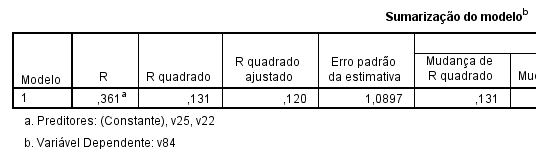
\includegraphics[height=4cm]{images/rl_ajustamento}
			\end{figure}

		\subsubsection{Teste t}

			Verifique a nulidade das variáveis.
			
			Caso exista, uma opção é retirar as variáveis nulas e rodar o modelo de novo. Outra opção é rodar uma regressão fatorial.

			É possível manter a variável mesmo nula caso ela seja muito importante para o modelo. \cite{torres}

			\begin{figure}[H]
				\centering
				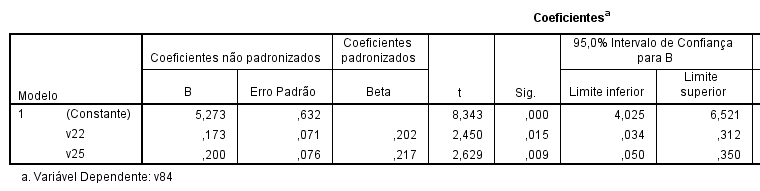
\includegraphics[height=4cm]{images/rl_teste-t}
			\end{figure}

		\subsubsection{Teste F}

			Ao verificar os resultados da ANOVA (\emph{Analysis of Variance}), veja se o sigma de F está abaixo de $ 5\% $ (caso seja esse o nível de significância desejado).

			\begin{figure}[H]
				\centering
				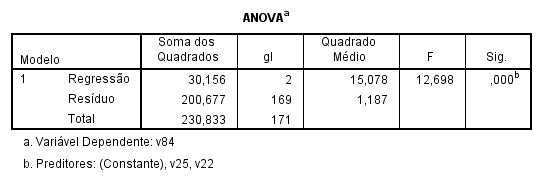
\includegraphics[height=4cm]{images/rl_anova}
			\end{figure}

			As premissas dos testes de hipóteses de F são as mesma do teste t. Seguem elas abaixo.

			\bigskip

			$
				\begin{cases}
					\mathsf{H}_{0} : & R^{2} = 0 \\
					\mathsf{H}_{a} : & R^{2} \neq 0
				\end{cases}
			$	

		\subsubsection{Normalidade dos Resíduos}

			É importante olhar a normalidade dos resíduos para verificar se eles estão ajustados ao modelo (neste caso linear) e também para verificar a presença/ausência de outliers.
			
			No SPSS isso se faz explorando a explorando os \textbf{resíduos standardizados Z} ou \emph{Standardized Residual Z - ZRE}. \cite{torres}

			\begin{figure}[H]
				\centering
				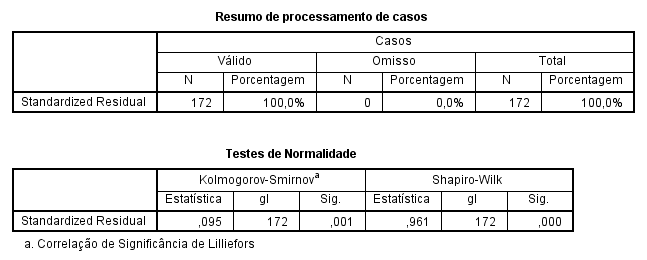
\includegraphics[height=6cm]{images/rl_normalidade-de-residuos}
			\end{figure}

		\subsubsection{Homocedasticidade dos Resíduos (Variância Constante)}

			``A presença de variâncias não homogêneas é uma violação de um dos pressupostos da regressão, conhecida como heterocedasticidade.
			
			\bigskip
			
			\textbf{Possíveis causas}: outliers; erro de especificação das variáveis; \textbf{erro na função matemática} (Ela pode ser não-linear. No marketing as disciplinas não passam por regressão não-linear, logo, nos exercícios a opção nunca será essa. O correto é testar outros modelos antes de retirar os outliers.), entre outros.
			
			\bigskip
			
			\textbf{Soluções possíveis}: transformar variáveis ou estimação da regressão via mínimos quadrados ponderados; retirada de outliers". \cite{torres}

			\bigskip

			Para analisar a homocedasticidade no SPSS, \textbf{gere um gráfico de dispersão simples} com a variável \emph{Studentized Residual - SRE} no eixo $ x $ e a variável \emph{Standardized Predicted Value - ZPR} no eixo $ y $ .

			\begin{figure}[H]
				\centering
				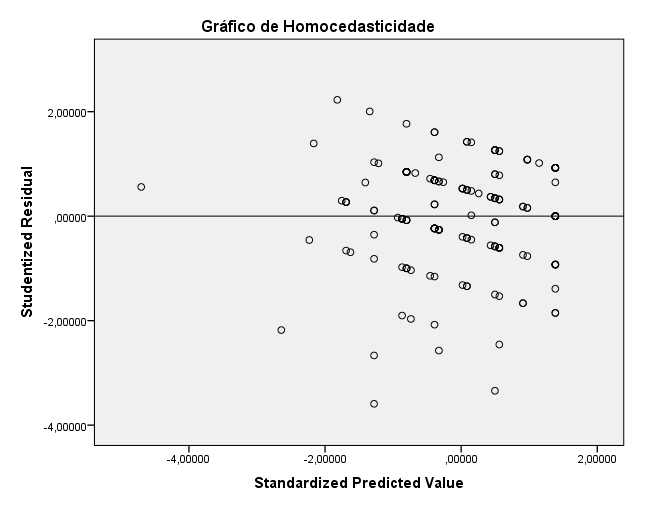
\includegraphics[height=6cm]{images/rl_homocedasticidade}
			\end{figure}

		\subsubsection{Linearidade}

			O diagnóstico de linearidade pode ser feito pelo diagrama de dispersão [o mesmo realizado para a avaliação de homocedasticidade, que dá uma boa ideia sobre sua linearidade em torno das observações das variáveis dependentes e independentes.

			\bigskip
			
			Suas possíveis causas e soluções são as mesmas apresentadas para Variância Constante (pressuposto anterior).

		\subsubsection{Ausência de Autocorrelação dos Resíduos}

			``A análise da autocorrelação dos resíduos pode ser feita através do Teste de Durbin-Watson, cujas hipóteses são:
			
			\bigskip

				$
					\begin{cases}
					\mathsf{H}_{0} : & \text{não existe autocorrelação dos resíduos} \\
					\mathsf{H}_{a} : & \text{existe autocorrelação dos resíduos}
					\end{cases}
				$

			\bigskip

			Quero que não exista autocorrelação, pois a violação leva a erro na estimação dos parâmetros.
			
			\bigskip
			
			A idéia da chamada autocorrelação serial é que os resíduos
contém mais informação sobre a variável dependente do que aquilo que foi “filtrado” pelas variáveis explicativas. Em termos técnicos, o resíduo ainda pode ser sistematizado.

			\bigskip

			Exemplos de autocorrelação são normalmente encontrados em trabalhos que utilizam séries de tempo como dados de análise.
			
			\bigskip
			
			A autocorrelação dos resíduos depende do valor do teste de Durbin-Watson, cuja interpretação é:
			
			\bigskip
			
			\textbf{Valores próximos de 2, não existe autocorrelação dos resíduos;}
			
			\bigskip
			
			Valores próximos de Zero, significa autocorrelação positiva;
			
			Valores próximos de 4, significa autocorrelação negativa". \cite{torres}

			\begin{figure}[H]
				\centering
				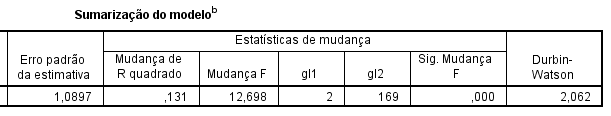
\includegraphics[height=3cm]{images/rl_durbin-watson}
			\end{figure}

		\subsubsection{Ausência de Multicolinearidade entre as Variáveis Independentes}

			``A multicolinearidade ocorre quando duas ou mais variáveis independentes do modelo apresentam \textbf{correlação alta (superiores em termos absolutos a 0,9)}, pois significa que contêm informações similares.
			
			\bigskip
			
			As consequências são: erros-padrão maiores, menor eficiências dos estimadores, estimativas imprecisas, entre outras". \cite{torres}

			\begin{figure}[H]
				\centering
				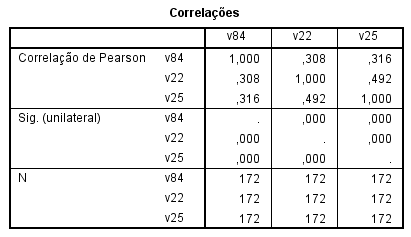
\includegraphics[height=5cm]{images/rl_multicolinearidade}
			\end{figure}

	\subsection{Análise de Outlier}
	
		``A identificação de outliers no modelo de regressão linear é feita essencialmente através dos \textbf{resíduos standardizados} (\emph{Standardized Residual - ZRE}), \textbf{studantizados} (\emph{Studentized Residual - SRE}) e \textbf{studantizados deletedos} (\emph{Studentized Deleted Residual - SDR}), pela verificação de pelo menos uma das condições:

		\begin{enumerate}[label=(\alph*)]
		
			\item Resíduos standardizados terem valores absolutos superiores a 3;			
			\item Resíduos studantizados terem valores absolutos superiores a 2;
			\item resíduos studantizados deleted terem valores absolutos superiores a 2". \cite{torres}
			
		\end{enumerate}

		Para isso gere \textbf{gráficos de linha simples} com as variáveis acima mencionadas com as seguintes configurações:
			
		Escala do gráfico: Mínimo: -4; Máximo: 4; Incremento: 1;

		Linhas de referências no eixo Y: ZRE: 3 e -3; SRE e SDR: 2 e -2.
			
		\begin{figure}[H]
			\centering
			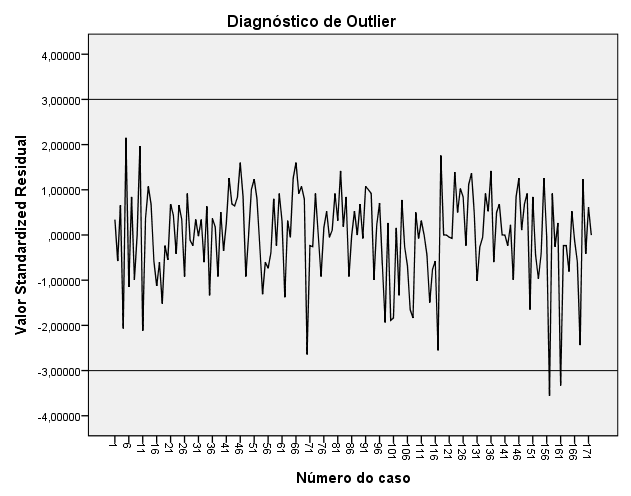
\includegraphics[height=6cm]{images/rl_analise-outlier_ZRE}
			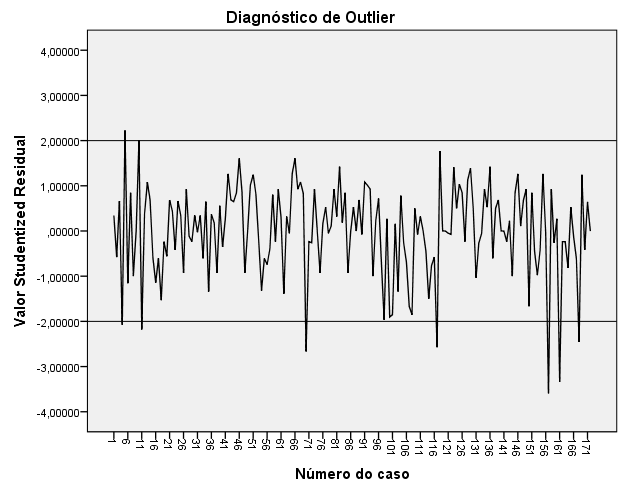
\includegraphics[height=6cm]{images/rl_analise-outlier_SRE}
			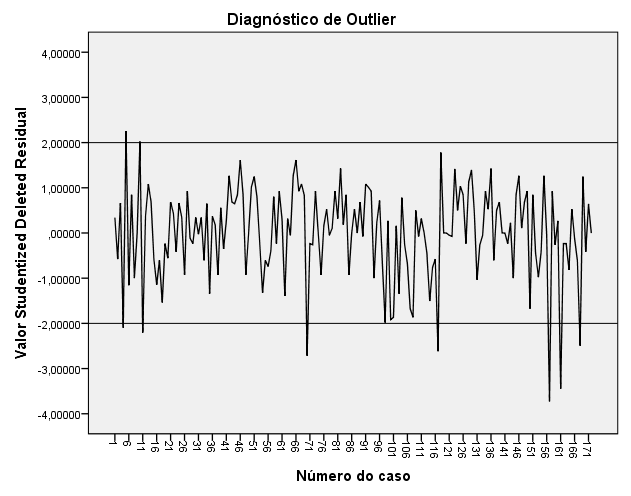
\includegraphics[height=6cm]{images/rl_analise-outlier_SRD}

		\end{figure}
			
		\textbf{Como remover os Outliers}

		\bigskip
				
		Comece tirando os outllies que aparecerem mais de um vez OU aqueles que a distância da linha de referência for maior - retire do $ n $ de número maior para o menor. Isso é importante pois o SPSS altera o número das linhas conforme você deleta o outlier.

		Rode o modelo de novo e veja se melhorou. Se não, retire mais outliers e repita o processo.

		Se você tirar muitos outliers você pode acabar com seu banco de dados. Caso isso aconteça um outra solução deve ser aplicada. Pode ser que colocando mais variáveis esse outliers melhorem (PODE SER).
	
	\section{Análise de Variância (ANOVA)}

	``A ANOVA é empregada para verificar se há diferença sistemática entre as médias de resultados \textbf{normalmente distribuídos} de experimentos randômicos.
	
	Trata-se de um método estatístico, que por meio de
\textbf{teste de igualdade de médias}, verifica se fatores (variáveis independentes) produzem mudanças sistemáticas em alguma variável de interesse (variável dependente).

	Os fatores propostos podem ser variáveis quantitativas
ou qualitativas, enquanto a variável dependente deve ser quantitativa.

	Todos os sujeitos (participantes ou unidades experimentais) de determinado grupo recebem o mesmo tratamento, assegurando que as diferenças sistemáticas entre médias de grupos possam ser atribuídas aos efeitos dos diferentes tratamentos" \cite{torres} .

	\subsection{Pressupostos da ANOVA \cite{torres}}

			\subsubsection{As observações dentro de cada grupo têm distribuição normal}
			
				``A normalidade não é restritiva ao uso da ANOVA quando o número de elementos em cada grupo é relativamente elevado $(n \geq 30)$ ;

				A não normalidade tem consequências mínimas na interpretação dos resultados, a não ser que a distribuição seja muito viesada".

				\textbf{Outras Observações}

					A normalidade é função da combinação de 2 medidas: assimetria e curtose. Se ela é normal ela é simétrica e meso-cúrtica;

					Caso ela não dê normal, uma possibildiade é calcular assimetria e a curtose. Então se divide as duas pelo desvio padrão;

					Se for normal, a divisão da assimetria/desvio padrão e curtose/desvio padrão deve ficar entre $ (-1,96 ; 1,96) $.

			\subsubsection{As observações são independentes entre si}
				Se as observações foram coletadas de maneira independente, logo os tratamentos serão independentes entre si (e.g. grupo experimental x grupo de controle).			
			
			\subsubsection{As variâncias de cada grupo são iguais entre si, \\ ou seja, há homocedasticidade}
			
				``O teste F é robusto a violações de homocedasticidade quando o número de observações em cada grupo é igual ou aproximadamente igual (considera-se grupos de dimensões semelhantes quando o quociente entre a maior dimensão e a menor for inferior a 1,5 - \textbf{se a razão entre a amostra de tamanho maior dividido pela amostra de tamanho menor der até 1,5 = OK});

				Quando os $ n $ não são iguais ou semelhantes e há grande afastamento tanto da normalidade como da homocedasticidade, põe-se em risco as conclusões tidas na análise de variância. Nesta situação recomenda-se utilizar testes alternativos não paramétricos de Kruskal-Wallis".

	\subsection{Cálculo da ANOVA}

		\subsubsection{Quadro da ANOVA}

			\begin{table}[H]

				\centering
		
				\begin{tabularx}{\textwidth}{X <{\centering} X <{\centering} X <{\centering} X <{\centering} X <{\centering}}
			
					Fonte de & Soma dos & Grau de & Quadrados & \multirow{2}{*}{Teste F} \\
				Variação & Quadrados & Liberdade & Médios \\
				
					\noalign{\smallskip} \hline \noalign{\smallskip}
				
					Entre & \multirow{2}{*}{$ Q_{e} $} & \multirow{2}{*}{$ k -1 $} & \multirow{2}{*}{$ S^{2}_{e} = \cfrac{Q_{e}}{k - 1} $} & \multirow{7}{*}{$ F_{\text{cal}} = \cfrac{S^{2}_{e}}{S^{2}_{r}} $} \\
					Tratamentos & & & & \\
				
					\noalign{\smallskip} \cline{1-4} \noalign{\smallskip}
				
					Dentro das & \multirow{3}{*}{$ Q_{r} = Q_{t} - Q_{e} $} & \multirow{3}{*}{$ n - k $} & \multirow{3}{*}{$ S^{2}_{r} = \cfrac{Q_{t} - Q_{e}}{n - k} $} & \\
					Amostras & & & & \\
					(Residual) & & & & \\
				
					\noalign{\smallskip} \cline{1-4} \noalign{\smallskip}
				
					Total & $ Q_{t} $ & $ n - 1 $ & &
				
				\end{tabularx}

			\end{table}

		\subsubsection{Fórmulas}
	
			\paragraph{Soma dos Quadrados Totais}
		
				{\Large $ Q_{t} = \sum \limits^{k}_{i=1} \sum \limits^{n_{i}}_{j=1} x^{2}_{ij} - C$}
			
			\paragraph{Soma dos Quadrados Entre Tratamentos}
		
				{\Large $ Q_{e} = \sum \limits_{i} \begin{bmatrix} \cfrac{ \begin{pmatrix} \sum \limits_{j} x_{ij} \end{pmatrix}^{2}}{n_{i}} \ \ \end{bmatrix} - C$}
			
			\paragraph{Constante}
		
				{\Large $ C = \cfrac{\begin{pmatrix} \sum \limits^{k}_{i=1} \sum \limits^{n_{i}}_{j=1} x_{ij} \end{pmatrix}^{2}}{n} $ }
			
		\subsubsection{Tabela de Contingência \cite{bussab}}
	
			\begin{table}[H]
				\centering
		
				\begin{tabularx}{\textwidth}{X <{\centering} X <{\centering} X <{\centering} X <{\centering} X <{\centering} X <{\centering} X <{\centering}}
			
					\multirow{2}{*}{Indivíduo} & \multicolumn{6}{>{\hsize=6\hsize\centering}X}{Variável} \tabularnewline
				& $ X_{1} $ & $ X_{2} $ & \dots & $ X_{j} $ & \dots & $ X_{p} $ \tabularnewline
				
					\noalign{\smallskip} \hline \noalign{\smallskip}
				
					1 & $ X_{11} $ & $ X_{12} $ & \dots & $ X_{1j} $ & \dots & $ X_{1p} $ \tabularnewline
				
					\noalign{\smallskip} \hline \noalign{\smallskip}
				
					2 & $ X_{21} $ & $ X_{22} $ & \dots & $ X_{2j} $ & \dots & $ X_{2p} $ \tabularnewline
				
					\noalign{\smallskip} \hline \noalign{\smallskip}
				
					. & . & . &  & . &  & . \tabularnewline
					. & . & . &  & . &  & . \tabularnewline
					. & . & . &  & . &  & . \tabularnewline

					\noalign{\smallskip} \hline \noalign{\smallskip}
				
					i & $ X_{i1} $ & $ X_{i2} $ & \dots & $ X_{ij} $ & \dots & $ X_{ip} $ \tabularnewline
				
					\noalign{\smallskip} \hline \noalign{\smallskip}
				
					. & . & . &  & . &  & . \tabularnewline
					. & . & . &  & . &  & . \tabularnewline
					. & . & . &  & . &  & . \tabularnewline
				
					\noalign{\smallskip} \hline \noalign{\smallskip}
				
					n & $ X_{n1} $ & $ X_{n2} $ & \dots & $ X_{nj} $ & \dots & $ X_{np} $ \tabularnewline
				
				\end{tabularx}

			\end{table}
		
		\subsubsection{Utilizando a Distribuição F (Fisher–Snedecor) para Testar a Nulidade dos Estimadores}
	
			``A distribuição “F” é apropriada para a \textbf{razão das variâncias de duas amostras}, tomadas independentemente da mesma população normalmente distribuída.

			A estatística usada para testar a hipótese nula de que não existe diferença entre as variâncias é " \cite{torres}:
		
			{\Large $ F_{v_{1},v{2}} = \cfrac{S^{2}_{1}}{S^{2}_{2}} \ , \ \text{onde} \ F_{v_{1},v{2}, \text{inferior}} = \cfrac{1}{F_{v_{2},v{1}, \text{superior}}} $}
		
			\paragraph{Teste de Hipóteses}

				$
					\begin{cases}
			        \mathsf{H}_{0} : & \mu_{A} = \mu_{B} = \mu_{C} \\
			        \mathsf{H}_{a} : & \text{As médias de pelo menos dois grupos são diferentes}
			        \end{cases}
				$
		
			\paragraph{Ponto crítico}
		
				$ F_{c} \ \alpha - 1 \ ; \ k - 1 \ ; \ n - k = ?  $
		
			\paragraph{Distribuições F \cite{google}} \hspace{0cm}
		
				\begin{figure}[H]
					\centering			
					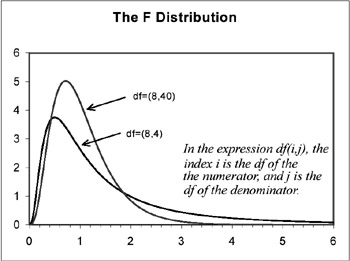
\includegraphics[height=6cm]{images/anova_distribuicao-f}
				\end{figure}					
					
	\subsection{ANOVA 1 Fator no SPSS \cite{torres}}

		Para executar a ANOVA no SPSS vá em ``Analisar $>$ Comparar Médias $>$ Análise de Variância Unidirecional...", porém não esqueça de verificar a normalidade dentro de cada grupo.

		Para verificar a normalidade utilizando o SPSS, faça os testes de Kolmogorov-Smirnov (\textbf{K-S}) e \textbf{Shapiro-Wilks} (verifique as hipóteses desses testes na seção de Regressão Linear).

		\subsubsection{Teste de Levene}

			O teste de Levene serve para verificar a homocedasticidade dentre os grupos, ou seja, se as variâncias de cada grupo são iguais entre si. ``Ele é tão sensível à violações de normalidade como o Teste de Bartlett. Porém, quando os “n” são iguais em cada grupo, a ANOVA é robusta às violações da homocedasticidade e o Teste de Levene se torna pouco útil" \cite{torres}.

			Caso não haja homocedasticidade, olhe o tamanho das amostras. Se elas não forem de tamanhos iguais ou semelhantes, não há teste paramétrico alternativo para utilizar.

			\bigskip

			\textbf{Teste de Hipóteses}

					\bigskip

					$
					\begin{cases}
						\mathsf{H}_{0} : & \text{As variâncias dentro dos grupos são homogêneas} \\
						\mathsf{H}_{a} : & \text{As variâncias dentro dos grupos não são homogêneas}
					\end{cases}
					$
			
			\bigskip \bigskip
			
			\textbf{Tabela}
			
				\begin{figure}[H]
					\centering			
					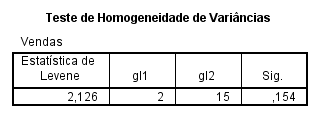
\includegraphics[height=3.5cm]{images/anova_levene}
				\end{figure}
				
		\subsubsection{Teste de Tukey}

			O teste de Tukey é um dos testes de comparação de médias mais utilizados por ser bastante rigoroso. Ele não permite comparar grupos entre si e é utilizado para testar toda e qualquer diferença entre duas médias de tratamento. É aplicado quando o teste $ F $ para tratamentos (1, 2, 3, ...) da ANOVA é significativo.

			\bigskip
			
			\textbf{Tabela}	

				\begin{figure}[H]
					\centering			
					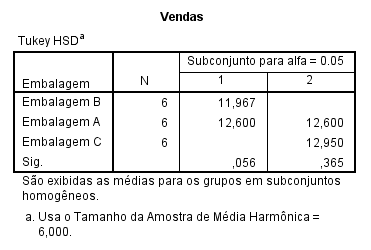
\includegraphics[height=7cm]{images/anova_tukey}
				\end{figure}

				O teste separa as médias dos grupos em subconjuntos. Quando dois ou mais grupos se encontram no mesmo subconjunto isso mostra que suas médias são iguais - a partir do nível de significância ($ \alpha $) aplicado.

				Neste caso, as embalagens A e B são iguais, assim como A e C, mas as embalagens B e C são diferentes, pois elas não aparecem juntas em nenhum subconjunto.

				A depender do que está sendo analisado, escolhe-se o tratamento ($ k $) que se destaca mais (não é igual aos outros) e que melhor se aplica à investigação (neste caso a embalagem C, pois sua média de vendas é maior do que A).
				
		\subsubsection{Tabela de Comparações Múltiplas}

			A tabela de comparações múltiplas compara as médias de diferentes tratamentos. Os testes seguem as seguintes hipóteses:

			\bigskip

			$
			\begin{cases}
				\mathsf{H}_{0} : & \mu_{1} = \mu_{2} \\
				\mathsf{H}_{a} : & \mu_{1} \neq \mu_{2}
			\end{cases} \hspace{1cm}			
			\begin{cases}
				\mathsf{H}_{0} : & \mu_{1} = \mu_{3} \\
				\mathsf{H}_{a} : & \mu_{1} \neq \mu_{3}
			\end{cases} \hspace{1cm}
			\begin{cases}
				\mathsf{H}_{0} : & \mu_{2} = \mu_{1} \\
				\mathsf{H}_{a} : & \mu_{2} \neq \mu_{1}
			\end{cases} \hspace{1cm}
			\begin{cases}
				\mathsf{H}_{0} : & \mu_{2} = \mu_{3} \\
				\mathsf{H}_{a} : & \mu_{2} \neq \mu_{3}
			\end{cases}
			$
			
			\bigskip

			E por ae vai, comparando todos os tratamentos entre si.

			\bigskip
			
			\textbf{Tabela}
			
			\begin{figure}[H]
				\centering		
				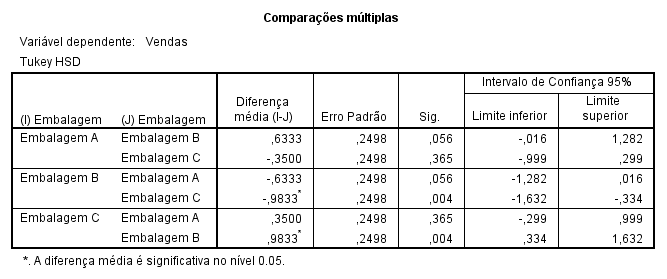
\includegraphics[height=7cm]{images/anova_comparacoes-multiplas}
			\end{figure}
			
			Neste caso podemos verificar que as médias de B e C são diferentes entre si, pois a significância é menor que 5\% ($ \alpha < 0.05$).

		\subsubsection{Tabela ANOVA}

			A tabela ANOVA comparada as médias dos grupos estudados, conforme já descrito mais acima. As hipóteses utilizadas são:

			\bigskip

			$
			\begin{cases}
				\mathsf{H}_{0} : & \mu_{1} = \mu_{2} = \mu_{3} \\
				\mathsf{H}_{a} : & \text{as médias de pelo menos dois grupos são diferentes}
			\end{cases}
			$
			
			\bigskip

			Ela pode analisar dois ou mais tratamentos. A lógica é sempre a mesma.

			\bigskip
			
			\textbf{Tabela}
			
			\begin{figure}[H]
				\centering
				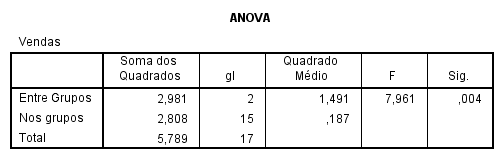
\includegraphics[height=4.5cm]{images/anova_tabela}
			\end{figure}						
			
			Neste caso rejeitamos a hipótese nula, pois a significância é menor que 5\% ($ \alpha < 0.05$).

	\subsection{ANOVA 2 Fatores \cite{torres}}

		``Sendo uma extensão da ANOVA, a ANOVA dois fatores permite analisar modelos de efeitos fixos ou mistos, analisar as tendências dos dados, proceder comparações múltiplas, analisar o efeitos das variáveis e controlar variáveis externas (fatores de segmentação da amostra)".
		É necessário primeiro fazer a ANOVA 1 fator para cada fator e seus tratamentos, antes de fazer uma ANOVA de 2 (ou mais) fatores, para verificar se os pressupostos da ANOVA estão satisfeitos.

		\bigskip

		\textbf{Teste de Hipóteses}

			\bigskip

			$
				\begin{cases}
					\mathsf{H}_{0} : & \text{não existe interação entre os fatores} \\
					\mathsf{H}_{a} : & \text{existe interação entre os fatores}
				\end{cases}
			$

	\subsection{ANOVA 2 Fatores no SPSS \cite{torres}}

		Para realizar a ANOVA 2 fatores no SPSS vá em Analisar $>$ Modelo linear geral $>$ Univariado.

		\subsubsection{Passo a Passo}

			\begin{figure}[H]
			
				\centering
				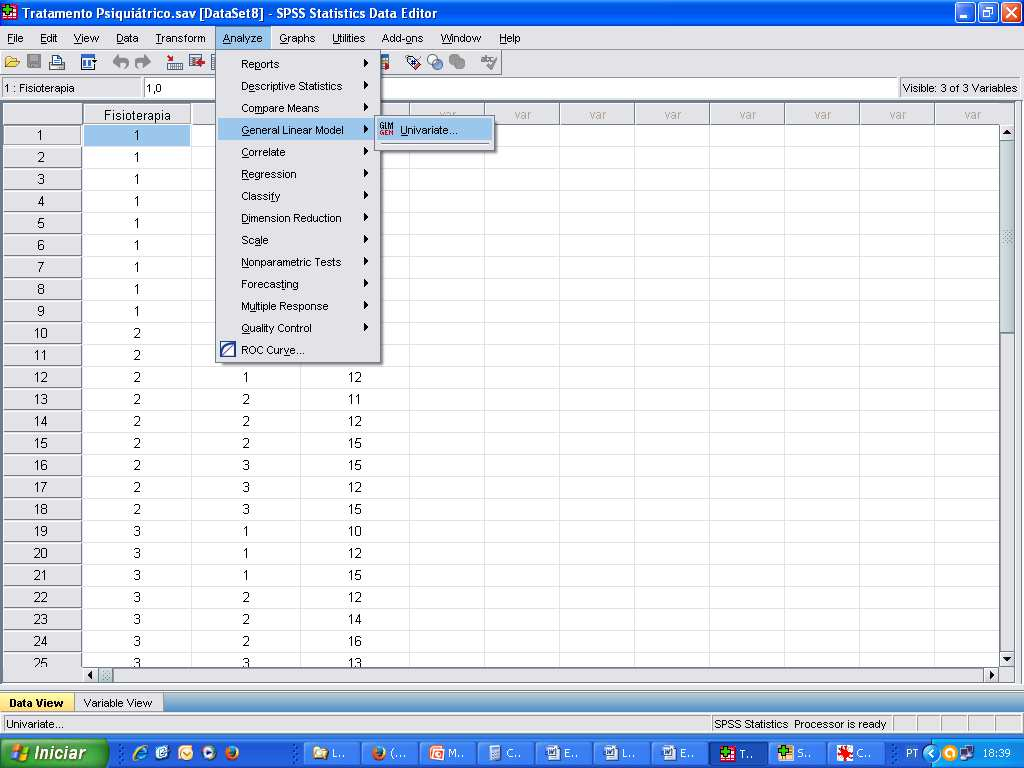
\includegraphics[height=8cm]{images/anova2_passo-a-passo_1}
			\end{figure}			
			
			\begin{figure}[H]
			
				\centering
				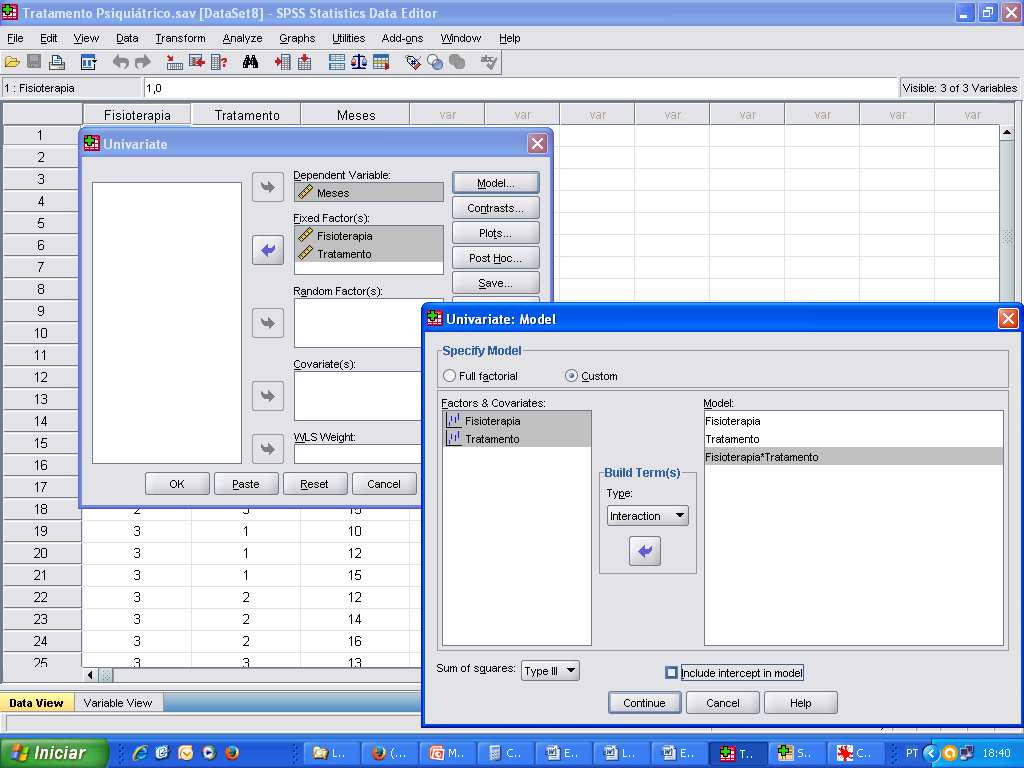
\includegraphics[height=8cm]{images/anova2_passo-a-passo_2}
			\end{figure}
			
			\begin{figure}[H]
			
				\centering
				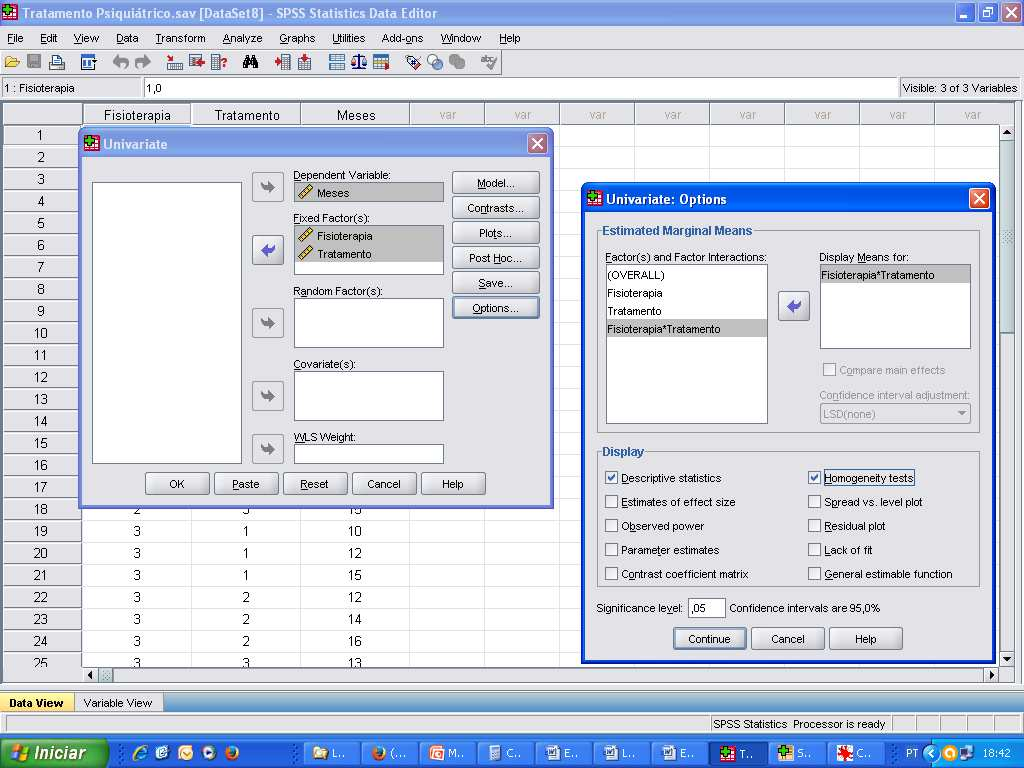
\includegraphics[height=8cm]{images/anova2_passo-a-passo_3}
			\end{figure}
		\subsubsection{Análise}

			Primeiro verifique a homocedasticidade dente os fatores pelo teste de Levene.

			O teste de hipótese da ANOVA 2 fatores se encontra na tabela de "Testes de efeitos entre sujeitos". O que nos importa aqui é a interação entre os fatores ("Fator 1*Fator 2"), logo, verifique a significância da interação pelas hipóteses da ANOVA 2 fatores.
	
	\section{Análise Discriminante}

	``A análise discriminante é uma \textbf{técnica multivariada} que \textbf{cria funções discriminantes}, provenientes de combinações lineares das variáveis iniciais, que maximizam as diferenças entre as médias dos grupos e minimizam a probabilidade de classificações incorretas dos casos nos grupos.

	É aplicada quando a \textbf{variável dependente é qualitativa} (grupos) e as \textbf{variáveis independentes são quantitativas}. As variáveis dicotômicas, como sexo, podem também ser incluídas nas variáveis explicativas.

	A análise discriminante \textbf{tem por objetivo escolher as variáveis que distinguem os grupos}, de modo que, conhecendo-se as características de um novo caso, se possa prever a que grupo pertence.

	A análise discriminante pode ser usada também para validar a análise de cluster e confirmar os resultados da análise fatorial". \cite{torres}

	\subsection{Hipóteses}

		$
			\begin{cases}

				\mathsf{H}_{0} : & \text{Não há diferença. As variáveis não discriminam os objetos investigados} \\
				\mathsf{H}_{a} : & \text{Há diferença. As variáveis discriminam os objetos investigados}

			\end{cases}
		$

		\bigskip

		\textbf{Observações}

			Se as variáveis têm uma diferença de grandeza entre elas, será preciso então padronizá-las para que a análise discriminante não as discrimine por essa razão.

	\subsection{Pressupostos}

		\subsubsection{Cada grupo é uma amostra aleatória de uma população normal multivariada}

			``A sua violação pode levar a decisões incorretas, principalmente quando as amostras são pequenas. \textbf{Quando a violação da normalidade se deve apenas à não simetria da distribuição, a potência do teste não é afetada}, contrariamente ao que acontece se a \textbf{distribuição não for mesocúrtica} e, de forma mais acentuada, se for platicúrtica, caso em que devemos optar pela regressão logística". \cite{torres}

			Para medir a curtose, divida a "estatística" pelo "erro padrão" (SPSS). Para verificar se ela é mesocúrtica, veja se o valor fica entre $-1,96 < x > +1,96$ . (Padronização Z: $1,96 = 0,475$ $\rightarrow$ 95\% no total (bicaudal)).

			Verifique os outliers. A remoção de outliers pode aproximar as variáveis para a normal. Outliers moderados não costumam criar grande impacto nas análises.

		\subsubsection{Dentro dos grupos a variabilidade é idêntica, isto é, as matrizes de variância e covariância são iguais para todos os grupos}

			Teste homocedasticidade, equivalente multivariado ao teste de Levene.

			``A verificação deste pressuposto é feita na própria análise discriminante, através do \textbf{teste Box’s M}. Caso seja violado, aumenta a probabilidade dos casos serem classificados no grupo com maior dispersão.

			A violação deste pressuposto afeta a análise principalmente quando os grupos não têm igual dimensão, mesmo que as diferenças sejam moderadas" \cite{torres}.

			\bigskip

			\textbf{Dicas e Recomendações \cite{torres}}

				\begin{itemize}
					\item O número mínimo de observações por variável independente: 5 ;
					\item Número recomendado de observações por variável: 20 ;
					\item Número de observações por grupo: o menor grupo deve ter um tamanho que exceda o número de variáveis independentes;
					\item É recomendável que o número mínimo de casos em cada grupo seja 20, e que os grupos tenham dimensões semelhantes.
				\end{itemize}
				
	\subsection{Análise Discriminante no SPSS \cite{torres}}

		\subsubsection{Teste M de Box(\textit{Box's M})}

			``Este teste verifica um dos pressupostos na análise discriminante (\textbf{pressuposto da homocedasticidade}). Ele testa se as diferentes dispersões são ou não estatisticamente significativas. É muito sensível a afastamentos da normalidade".

			O teste Box's M é muito ``sensível à desvios de normalidade e à dimensão das amostras (amostras grandes conduzem geralmente à rejeição de Ho)". Para solucionar uma possível violação do pressuposto da homocedasticidade  é importante ter uma amostra grande com o mesmo número de observações em cada grupo. ``Segundo alguns autores, a análise discriminante é uma técnica bastante robusta à violação dos pressupostos, desde que a \textbf{dimensão do menor grupo seja superior ao número de variáveis independentes em estudo}".

			\bigskip

			\textbf{Hipóteses}

				\bigskip

				$
					\begin{cases}

					\mathsf{H}_{0} : & \text{As matrizes observadas de variância-covariância são iguais entre grupos} \\
					\mathsf{H}_{a} : & \text{As matrizes observadas de variância-covariância não são iguais entre grupos}

					\end{cases}
				$

			\bigskip \bigskip

			\textbf{Tabela}

				\begin{figure}[H]
					\centering
					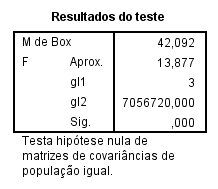
\includegraphics[height=5.5cm]{images/analise-discriminante_teste-box-s-m}
				\end{figure}
				
		\subsubsection{Teste Lambda de Wilks (\textit{Wilk's Lambda})}

			``O Wilk’s Lambda dá informação sobre as diferenças entre os grupos, para cada variável individualmente. Obtém-se pela razão entre a variação dentro dos grupos e a variação total.

			Este teste é robusto a violação do Teste Box’s M quando os grupos têm dimensões semelhantes.

			A não rejeição da hipótese de igualdade da média de uma variável nos grupos ($\alpha > 0,05$), aumenta a probabilidade de ser classificada incorretamente em outro grupo".

			\bigskip

			\textbf{Tabela de Estatísticas de Grupo}

				Será que essas médias são significativamente diferentes (pela variabilidade das mesmas) ou elas podem ser consideradas iguais?

				\begin{figure}[H]
					\centering
					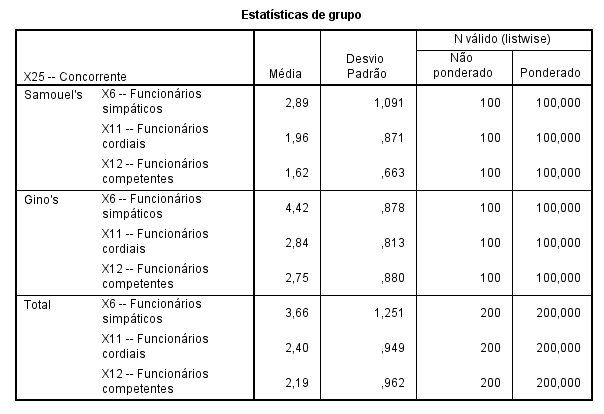
\includegraphics[height=10cm]{images/analise-discriminante_estatisticas-de-grupo}
				\end{figure}

			\textbf{Hipóteses}

				\bigskip

				$
					\begin{cases}

					\mathsf{H}_{0} : & \text{Não existe diferença entre as médias dos grupos} \\
					\mathsf{H}_{a} : & \text{Existe diferença entre as médias dos grupos}

					\end{cases}
				$

			\bigskip \bigskip

			\textbf{Tabela Lambda de Wilks}

				\begin{figure}[H]
					\centering
					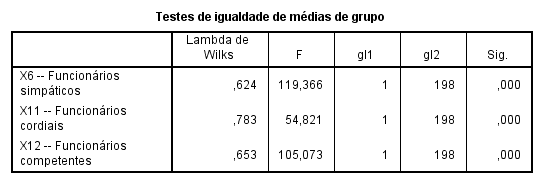
\includegraphics[height=5cm]{images/analise-discriminante_lambda-de-wilks}
				\end{figure}

				``Neste caso, como temos 3 variáveis, devemos comparar a significância com $\alpha / 3 = 0,05/3 = 0,017 $ e não com $\alpha = 0,05$. Como todas as significâncias são $< 0,017$, devemos rejeitar $\mathsf{H}_{0}$.

				A tabela mostra que existe diferenças significativas nas médias de cada variável nos dois grupos ($\text{significâncias} = 0,000$), não informando, entretanto, sua importância para discriminar grupos".

		\subsubsection{Contribuição das Variáveis}

			\paragraph{Matrizes intragupos em pool \textit{Pooled within-groups matrices}} \hspace{0cm}

				``Na sua interpretação tem de se levar em consideração a correlação entre as variáveis explicativas, pois se duas variáveis tiverem correlação $1$, incluir ambas não fornece mais informação do que incluir uma só. Por isso o uso da opção \textit{Stepwise}".

				\begin{figure}[H]
					\centering
					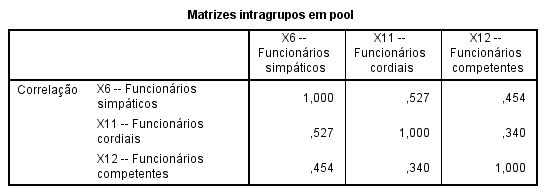
\includegraphics[height=5.5cm]{images/analise-discriminante_matrizes-intragupos-em-pool}
				\end{figure}

				Nessa tabela, "como podemos observar, não existe problema de \textbf{multicolinearidade}, uma vez que nenhum coeficiente de correlação entre variáveis independentes é superior, em termos absolutos, a $0,9$.

				Quando há multicolinearidade, não se deve analisar a importância de cada variável para a análise, visto que sua elevada correlação com outras a torna redundante. Nesta situação apenas se usa o procedimento \textit{Stepwise}".
				
			\paragraph{Estatísticas \textit{Stepwise}} \hspace{0cm}

				\begin{figure}[H]
					\centering
					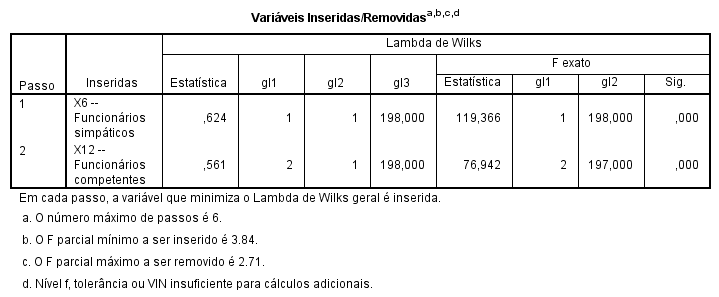
\includegraphics[height=6.5cm]{images/analise-discriminante_stepwise_var-inseridas-removidas}
				\end{figure}

				$
					\begin{cases}

					\mathsf{H}_{0} : & \text{A separação dos grupos não foi bem sucedida (em função das médias)} \\
					\mathsf{H}_{a} : & \text{A separação dos grupos foi bem sucedida (em função das médias)}

					\end{cases}
				$

				\bigskip \bigskip

				``A tabela acima resume o procedimento Stepwise, indicando para cada passo que variáveis foram adicionadas/removidas, o valor de Wilk’s Lambda e a significância. Note que a cada passo, a variável “escolhida” é aquela que minimize o valor de Wilk’s Lambda, isto é, aquela para a qual ocorrem maiores diferenças entre as médias dos grupos, até que não ocorram variação significativas de Lambda.

				O Teste Wilk’s Lambda avalia se o modelo consegue separar e classificar bem os grupos.

				Neste caso, com uma significância menor que $0,05$, podemos dizer que a separação dos grupos foi bem sucedida".

				\begin{figure}[H]
					\centering
					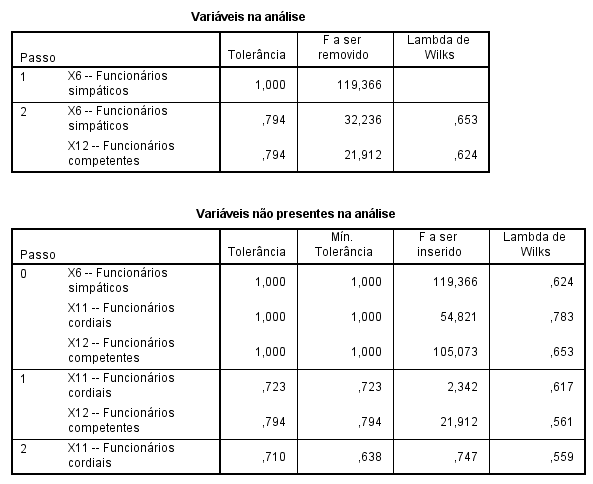
\includegraphics[height=13cm]{images/analise-discriminante_stepwise_var-presentes-e-n-presentes}
				\end{figure}

				``O quadro acima apresenta, para cada passo, as variáveis que foram consideradas como discriminantes na análise. Essas variáveis foram escolhidas como as “melhores”, com base na matriz de correlação, seu poder de discriminação entre grupos e cálculo da tolerância (avaliação da multicolinearidade. Valores muito baixos demonstrariam multicolinearidade).

			\paragraph{Sumarização de funções discriminantes canônicas} \hspace{0cm}

				\begin{figure}[H]
					\centering
					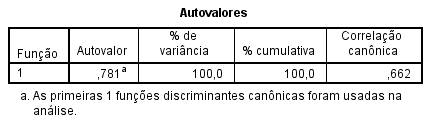
\includegraphics[height=3.5cm]{images/analise-discriminante_sumarizacao_autovalores}
				\end{figure}

				``A tabela acima indica que a variância (em termos da diferença entre os grupos) é explicada em 100\% pela função discriminante".

				\begin{figure}[H]
					\centering
					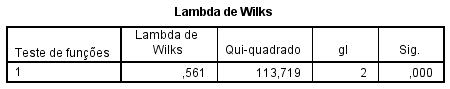
\includegraphics[height=2.5cm]{images/analise-discriminante_sumarizacao_lambda-de-wilks}
				\end{figure}

				$
					\begin{cases}

					\mathsf{H}_{0} : & \text{A função discriminante não é significativa} \\
					\mathsf{H}_{a} : & \text{A função discriminante é significativa}

					\end{cases}
				$

				\bigskip

				Neste caso ``a função discriminante é significativa para separar os grupos".

				\begin{figure}[H]
					\centering
					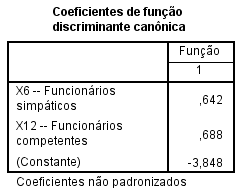
\includegraphics[height=6cm]{images/analise-discriminante_sumarizacao_coeficiente-de-funcao-d-c-}
				\end{figure}

				A tabela acima é "usada para escrever a(s) função(ões) discriminante(s)".

				\bigskip

				{\Large Função $= -3,848 + (0,642 * \mathsf{X}6) + (0,688 * \mathsf{X}12)$}

				\bigskip

				Considere $\mathsf{X}6 = 2$ e  $\mathsf{X}12 = 1$ $\rightarrow$ Função $= -1,8768$ $\rightarrow$ Pertence ao Samouel's (Olhe a tabela do centróide mais abaixo)

				\bigskip

				Considere $\mathsf{X}6 = 4$ e  $\mathsf{X}12 = 3$ $\rightarrow$ Função $= 0,7818$ $\rightarrow$ Pertence ao Gino's (Olhe a tabela do centróide mais abaixo)
				
			\paragraph{Estatísticas de classificação} \hspace{0cm}

				\begin{figure}[H]
					\centering
					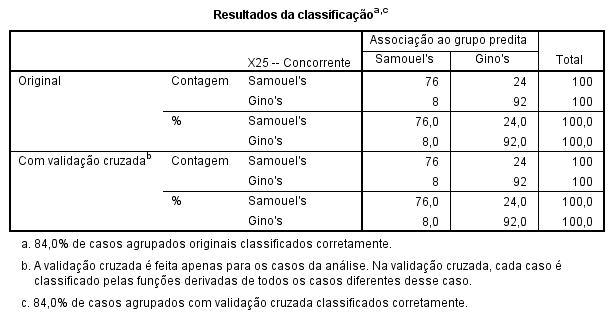
\includegraphics[height=8cm]{images/analise-discriminante_classificacao_resultados}
				\end{figure}

				``Finalmente, a tabela acima apresenta os resultados da classificação. Repare que 76\% dos clientes do Samouel's foram classificados corretamente e que 24\% dos clientes foram classificados como clientes do Ginos's. Além disso, 92\% dos clientes do Gino's foram classificados corretamente e 8\% não".

				\begin{figure}[H]
					\centering
					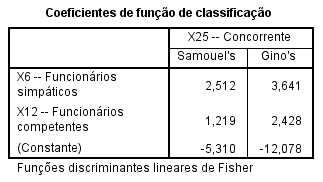
\includegraphics[height=5cm]{images/analise-discriminante_classificacao_coeficientes-de-funcao}
				\end{figure}

				A tabela acima é utilizada para escrever a(s) função(ões) para alocação dos dados.

				\bigskip

				{\Large Função Samouel's $= -5,310 + (2,512 * \mathsf{X}6) + (1,219 * \mathsf{X}12)$}

				\bigskip

				{\Large Função Gino's $= -12,078 + (3,641 * \mathsf{X}6) + (2,428 * \mathsf{X}12)$}

				\bigskip

				Condidere $\mathsf{X}6 = 2$ e  $\mathsf{X}12 = 1$

				\bigskip

				Função Samouel's $= -5,310 + (2,512 * 2) + (1,219 * 1) = 0,933$
				
				Função Gino's $= -12,078 + (3,641 * 2) + (2,428 * 1) = -2,368$

				\bigskip

				Condidere $\mathsf{X}6 = 4$ e  $\mathsf{X}12 = 3$

				\bigskip

				Função Samouel's $= -5,310 + (2,512 * 4) + (1,219 * 3) = 8,359$
				
				Função Gino's $= -12,078 + (3,641 * 4) + (2,428 * 3) = 9,77$

				\begin{figure}[H]
					\centering
					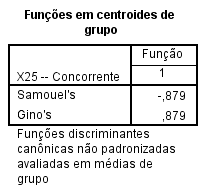
\includegraphics[height=6.5cm]{images/analise-discriminante_centroides-de-grupo}
				\end{figure}

				``Uma abordagem final para exame de diferenças entre grupos é o centróide. Em uma análise discriminante com dois grupos temos dois centróides, com três grupos três centróides, etc.

				Os centróides para nosso exemplo mostra que o do Samouel’s é $-0,879$ e do Gino’s $0,879$. Esta é uma medida de síntese global que indica que o Gino’s é percebido de maneira muito mais positiva do que o Samuel’s".

		\subsubsection{Passo a Passo}

			Não esqueça de verificar os pressupostos da análise antes de fazê-la.

			\begin{figure}[H]
				\centering
				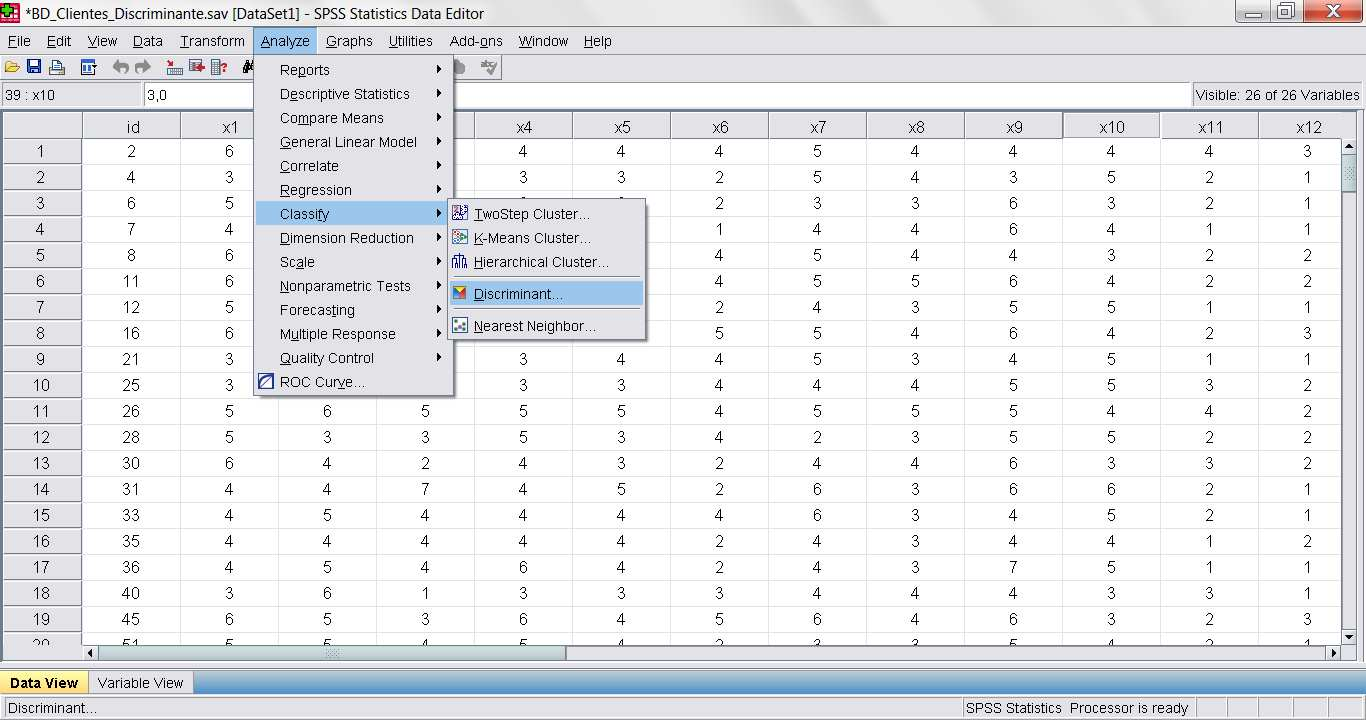
\includegraphics[height=8cm]{images/analise-discriminante_passo-a-passo_1}
			\end{figure}			
			
			\begin{figure}[H]
				\centering
				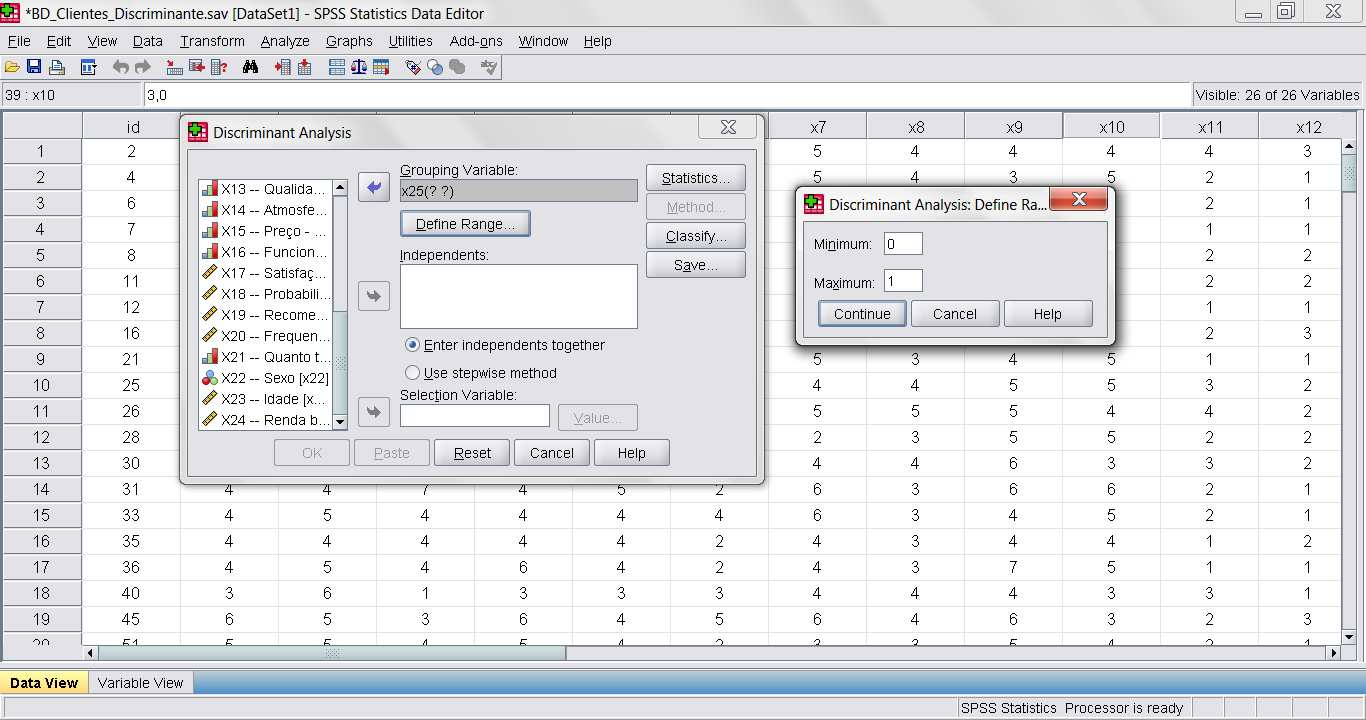
\includegraphics[height=8cm]{images/analise-discriminante_passo-a-passo_2}
			\end{figure}
			
			\begin{figure}[H]
				\centering
				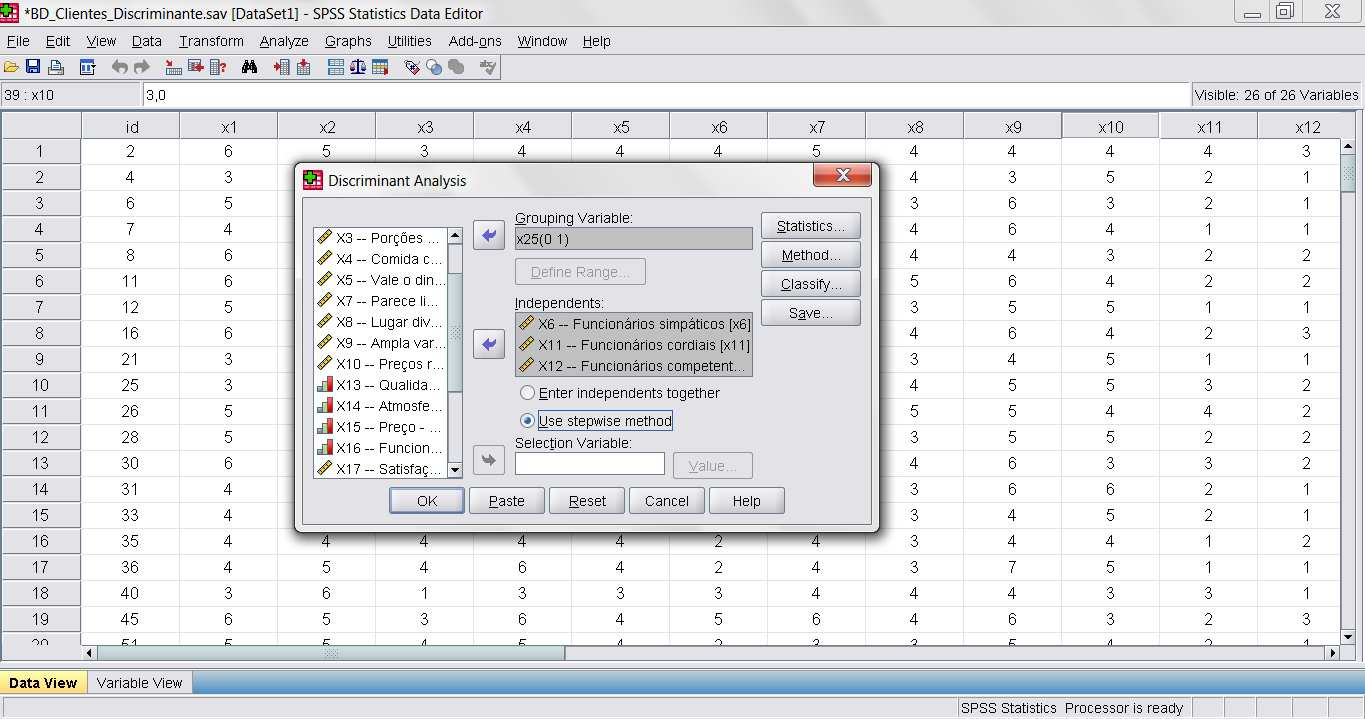
\includegraphics[height=8cm]{images/analise-discriminante_passo-a-passo_3}
			\end{figure}

			\begin{figure}[H]
				\centering
				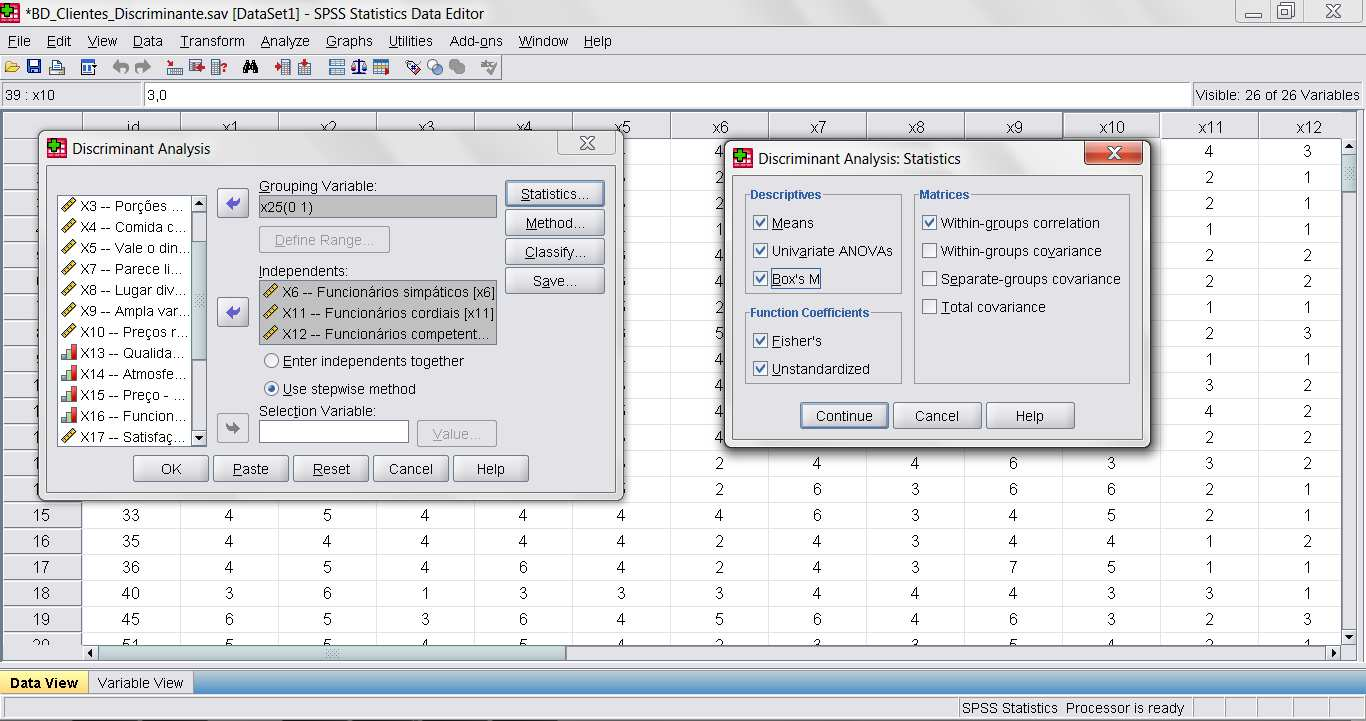
\includegraphics[height=8cm]{images/analise-discriminante_passo-a-passo_4}
			\end{figure}

			\begin{figure}[H]
				\centering
				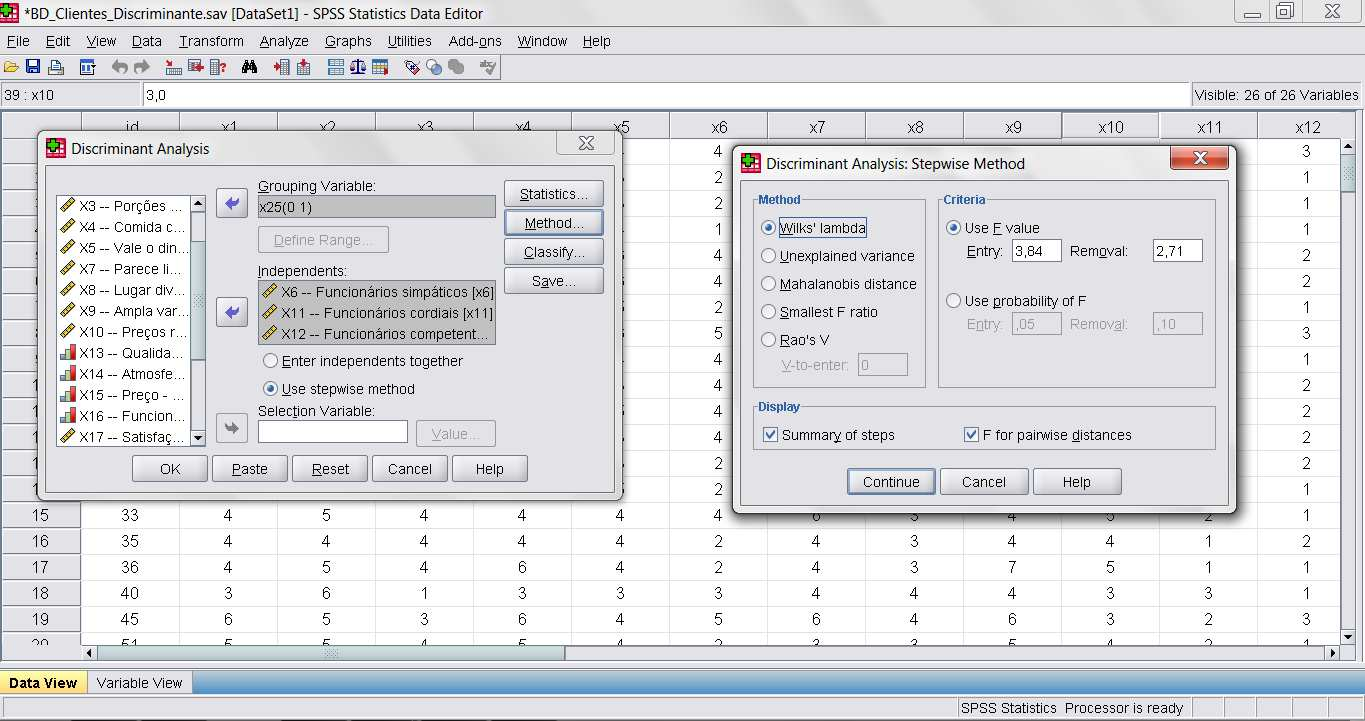
\includegraphics[height=8cm]{images/analise-discriminante_passo-a-passo_5}
			\end{figure}

			\begin{figure}[H]
				\centering
				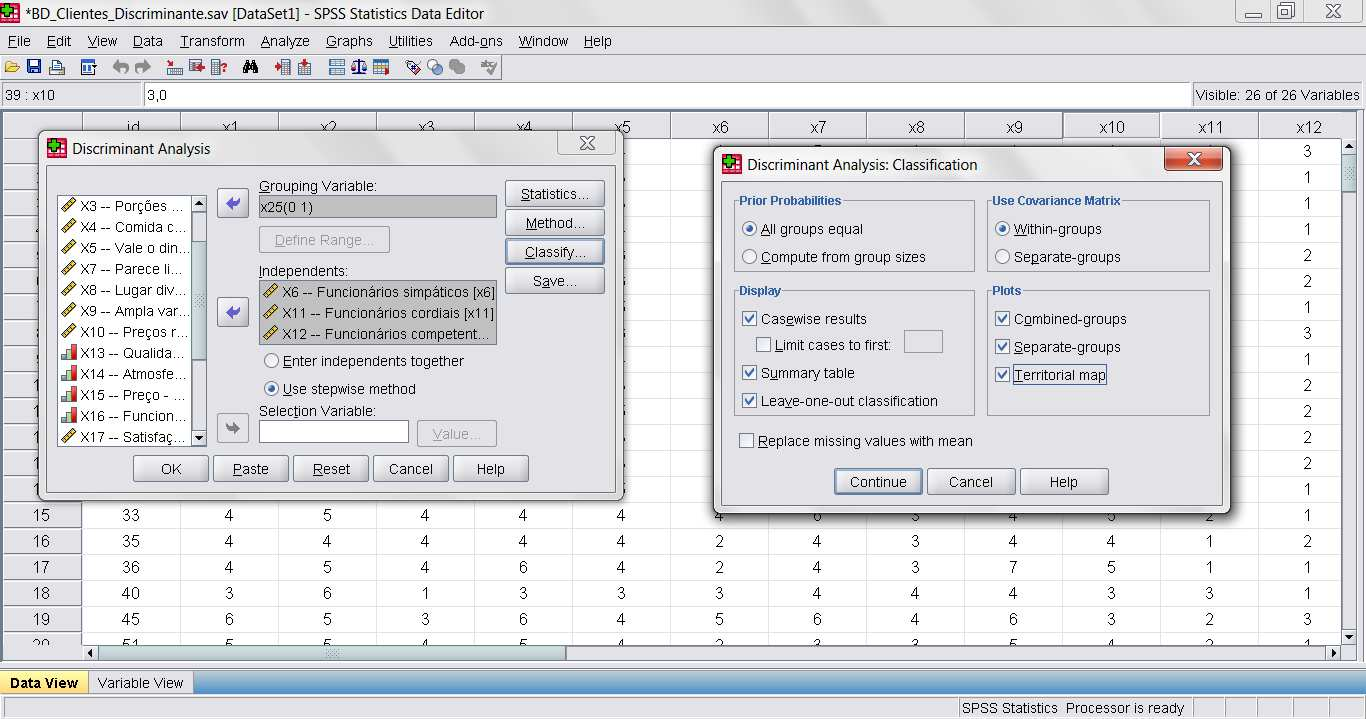
\includegraphics[height=8cm]{images/analise-discriminante_passo-a-passo_6}
			\end{figure}

			\begin{figure}[H]
				\centering
				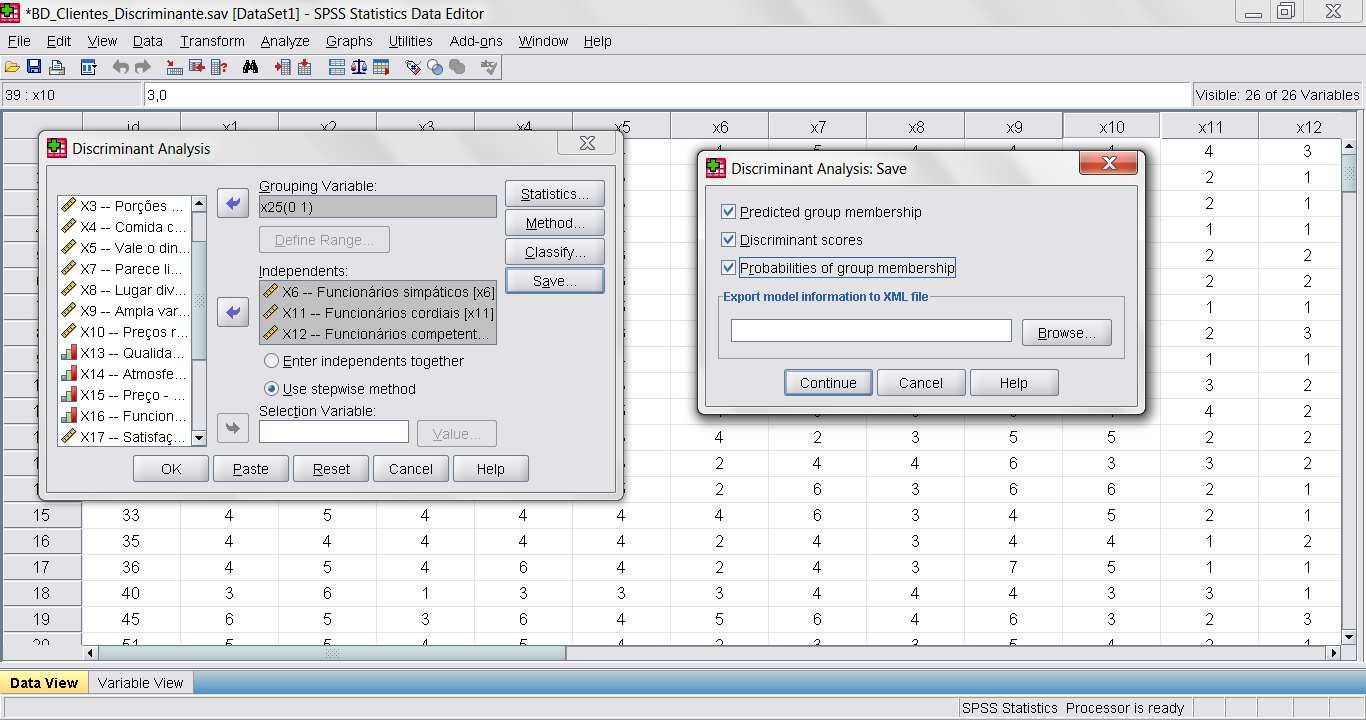
\includegraphics[height=8cm]{images/analise-discriminante_passo-a-passo_7}
			\end{figure}
	
	\section{Teoria da Amostragem \cite{torres}}

	$\overline{X} \pm Z * \sigma_{\overline{X}}$
	
	$\overline{X} \pm Z * cfrac{\sigma}{\sqrt{n}}$

	\subsection{Tamanho da Amostra}
	
	    \subsubsection{Amostra Aleatória Simples}
	    
	    Para estimar a média: com reposição
	    
	    Sabemos que $ Z $ (Erro amostral) $ = $ Erro absoluto, isto é:
	    
	    $Z_{x} \sigma_{\overline{X}} = e$ \\ onde \\ 
	    
	    ...
	    
	    
	
	    
	
	\section{Análise Fatorial \cite{torres}}

    (...)

	\subsection{O que é?}

        É o conjunto de técnicas estatísticas, que procura explicar a correlação entre as variáveis observáveis, simplificando os dados através da redução do número...
        
    \subsection{Objetivos}
    
        O objetivo principal da análise fatorial é a redução da massa de dados altamente relacionados. Entretanto, a redução não implica em admitir perda do comportamento das variáveis originais. Nesse sentido quer-se reduzir a massa de dados, mas ao mesmo tempo, preservar ao máximo as características comportamentais do conjunto de variáveis.
        
        A análise fatorial também é utilizada para gerar fatores compostos pelas variáveis originais, que podem ser utilizados em outras técnicas de análise multivariada.
        
        Como os fatores gerados em uma análise fatorial podem não apresentar correlação entre si, então podem ser utilizados para resolver o problema de variáveis multi-correlacionadas na regressão.
        
    \subsection{Dimensão da Amostra}
    
        O mínimo de respostas válidas ($N$) por variáveis ($K$) é:
        
        $
        N = 50 \text{se} K <= 5
        N = 10 * K se 5 < K <= 15
        N = 5 * K se K > 15
        $
        
        (Gráfico)
        
    \subsection{Análise Fatorial Exploratória e de Confirmação}
    
    \subsection{Exemplo:}
    
        Phil gostaria de saber se poderia simplificar seu entendimento das percepções dos dois restaurantes, reduzindo o número de variáveis para menos de 12 (tratar como amostra única). Isto é, se ele pode representar as 12 variáveis originais de percepção ($X_{1}$ até $X_{12}$) com um número menor de fatores significativos. A que resultados chegou o consultor?
        
        \subsubsection{Variáveis do banco de dados}
        
            \textbf{X1} - Comida de excelente qualidade
            
            \textbf{X2} - Um interior atraente
            
            \textbf{X3} - Porções generosas
            
            \textbf{X4} - Comida de gosto excelente
            
            \textbf{X5} - Bom valor para o dinheiro
            
            \textbf{X6} - Funcionários simpáticos
            
            \textbf{X7} - Aparência limpa e organizada
            
            \textbf{X8} - Um ambiente divertido
            
            \textbf{X9} - Grande variedade de pratos
            
            \textbf{X10} - Preços razoáveis
            
            \textbf{X11} - Funcionários gentis
            
            \textbf{X12} - Funcionários competentes
            
    \subsection{Premissas:}
    
        A análise fatorial possui algumas premissas:
        
        1a \textbf{As variáveis devem ser medidas em escala intervalar ou razão};
        
        2a As variáveis envolvidas na análise devem ser normalmente distribuídas;
        
        3a Se as variáveis envolvidas na análise estiverem medidas em escalas diferentes, as mesmas devem ser padronizadas antes de proceder a análise.
        
        \subsubsection{Quando os Dados não são Normais}
    
            Neste caso, devemos proceder da seguinte maneira: (1) usar uma transformação matemática que normalize a variável e usar a nova variável no lugar da original não normal; ou (2) alguns autores dizem que uma variável mesmo que não seja normalmente distribuída, pode ser incluída na análise fatorial, se apresentar simetria.
        
            Para verificar se as variáveis, mesmo não sendo normais, tem distribuição simétrica: calcular a assimetria e dividir (Stat/Std. Error). Se o valor estiver contido no intervalo [-1.96; 1,96] podemos supor que exista uma distribuição simétrica.
        
    \subsubsection{Próximo Passo}
        
    \subsection{Rotação de Fatores}
        
        A matriz de fatores contém os coeficientes utilizados para expressar as variáveis em termos dos fatores. Esses coeficientes, chamados de cargas fatoriais, representam as correlações entres os fatores e as variáveis. Um coeficiente com valor absoluto grande, indica que o fator e a avariável estão estritamente relacionados.
            
        Ao fazer a rotação dos fatores, seria interessante que cada variável tivesse coeficiente diferente de zero ou significativos com poucos fatores, sendo o ideal com apenas um, pois se vários fatores têm altas cargas com a mesma variável, tona difícil interpretá-los.
            
        \subsubsection{Tipo de Rotação de Fatores:}
            
            \textbf{Ortogonais}: rotação de fatores em que os eixos são mantidos em ângulos retos. A rotação ortogonal tem como resultado fatores não-correlacionados (varimax, quartimax e equamax). O mais utilizado é o varimax, que minimiza o número de variáveis com altas cargas sobre um fator, facilitando assim, a interpretação dos fatores.
                
            \textbf{Oblíquas}: rotação de fatores em que os eixos não são mantidos em ângulos retos. Deve-se utilizar rotação oblíqua quando os fatores na população tendem a ser fortemente correlacionados (direct oblimin e promax)
                
    \subsection{Tipos de Extração de Fatores:}
        
        \textbf{Componentes principais}: Geralmente usamos o padrão: \textbf{Análise de Componentes Principais}. No SPSS, bem como em outros pacotes de software de estatística, o PCA é o método padrão para a extração de análise fatorial. Ele não é especificamente um método de análise fatorial , mas é amplamente usado como um método de extração.
            
        É um procedimento estatístico multivariado, que permite transformar um conjunto de variáveis \textbf{quantitativas iniciais}, correlacionadas entre si, em outro conjunto com um menor número de variáveis não correlacionadas reduzindo a complexidade dos dados. \textbf{Não pressupõe a normalidade}, mas sua ausência ou presença de \textit{outliers} \textbf{pode} provocar distorções.
            
        As componentes principais são calculadas por ordem decrescente de importância, isto é, a primeira explica a máxima variâncias dos dados, segunda a máxima variância ainda não explicada pela primeira, e assim sucessivamente. A última componente será a que menos explica a variância total dos dados.
            
        \\
            
        \textbf{Máxima Verossimilhança}: a \textbf{normalidade é um pressuposto exigido} por esse método, isto é, ele assume que os dados provém de uma distribuição normal \textbf{multivariada}.
            
        Não é simplesmente fazer o teste de Komolgrov, é preciso calcular o teste "PK de Mardia" - que junto as variáveis em uma só e testa sua normalidade;
            
        \\
            
        \textbf{Eixo Principal de Fatoração ou Análise Fatorial Comum}: Opte pela Análise Fatorial Comum \textbf{se os seus dados são significativamente anormais}. Esse método de extração ...
        
    \subsection{KMO}
    
        Para se poder aplicar o modelo fatorial, deve haver correlação entre as variáveis. Se essas correlações forem pequenas é pouco provável que partilhem fatores comuns.
        
        O KMO é um procedimentto estatístico que permite aferir a qualidade das correlações entre as variáveis de forma a prosseguir com a análise fatorial
        
        ...
        
    \subsection{Teste de Esfericidade de Bartlett}
        
        O teste de Esfericidade de Bartlett testa a hipótese de que há correlação entre algumas variáveis.
        
        \textbf{Este teste requer que os dados provenham de uma população normal multivariada}. No entanto, este teste é muito influenciado pelo tamanhos da amostra, e eleva a rejeitar a hipótese nula em grandes amostras. Neste caso, é preferível o uso do KMO.
    
    \subsection{Extração de Fatores}
    
        O número de fatores necessários para descrever os dados, pode ser obtido através de um dos seguintes procedimentos:
        
        *K = número de variáveis.
        
        \\
        
        1. \textbf{para $K <= 30$}, usar o critério de Kaiser, pelo qual se escolhem os fatores cuja variância explicada é superior a 1 (eigenvalues $> 1$);
        
        \\
        
        2.\textbf{para $K > 30$}m usar o Scree Plot, isto é, o gráfico da variância pelo número de componente, onde os pontos no maior declive são indicativos do número apropriado de componentes a reter.
        
        \\
        
        Quando o número de casos é superior a 250 e o valor médio das comunalidades é grande ($>= 0,6$), ambos os critérios fornecem o mesmo resultado.
        
        Quando as comunalidades são pelo menos $0,6$ e o número de variáveis é inferior a 30 ou o número de observações é superior a 250, tanto o critério de Kaiser, como o Scree Plot, geram soluções confiáveis quanto ao número de fatores a reter. Essa credibilidade é aumentada quando o quociente entre o número de fatores retidos e o número de variáveis iniciais é inferior a $0,3$.
        
    \subsection{Matriz de Anti-Imagem}
    
        A matriz de anti-imagem é uma medida de adequação amostral de cada variável (MAS) para uso da análise fatorial onde pequenos valores (menores que $0,5$) na diagonal principal nos levam a considerar a eliminação da variável.
        
    \subsection{Comunalidade}
    
        Pelo quadro das comunalidades podemos observar que todas as variáveis possuem uma forte relação cpom os fatores encontrados, exceto as variáveis X7 e X10 que estão bem próximas do limite $0,6$.
        
    \subsection{Matriz de Componentes}
    
        A matriz dos componentes mostra as coeficientes ou pesos que correlacionam as variáveis aos fatores antes da rotação.
        
        Espera-se que não hajam pesos elevados, em mais de um fator, para uma mesma variável, pois isto dificultaria a interpretação. Muitas vezes a extração inicial ou anterior à rotação não fornece fatores interpretáveis.
        
        Na análise fatorial, quando há variáveis com baixos pesos, não se controla a sua influência eliminando-as e usando apenas as variáveis com pesos elevados. Cabe ao pesquisador excluí-las ou não da análise, de acordo com o fundamento teórico subjacente.
        
    \subsection{Matriz de Componentes após Rotação}
    
        A matriz dos componentes após a rotação ortogonal é útil para designar o significado dos fatores, essencialmente quando as variáveis têm pesos elevados ...
        
    \subsection{Nomeando os Fatores}
    
    ...
	
	\section{Alpha de Cronbach \cite{torres}}

	\subsection{Consistência Interna}
	
	    \subsubsection{O Que é?}
	
	        Consistência interna de um teste (ou questionário) é uma medida que vida detectar se os itens que o compões mede o mesmo conceito (ou constructo). Por exemplo, se dez questões foram projetos para medir o mesmo conceito, reo respondentes ...
	        
	        Para medir a consistência interna de um teste ou uma escala Lee J; Cronbach desenvolveu em 1951 o coeficiente alpha que hoje é a estatística ....
	        
	        ...
	        
	        As opões de resposta para cada item podem ser dicotômicas como "Sim" e "Não" ou escalonadas ...
	        
	        Seja $x_{ij}$ o i-ésimo...
	        
	        ...
	        
        \subsection{}
	

        
	
	\section{Análise de Cluster \cite{torres}}

	\subsection{O que é?}

        A análise de grupos ou de clusers, é uma técnica exploratória de análise multivariada que permite agrupar sujeitos ...
        
        A análise de cluster é um bom procedimento para exploração dos dados, quando eiste a suspeita de uqe a amostra não é homegênea.
        
    \subsection{Semelhanças}
    
        A análise de \textbf{cluster de variáveis} assemelha-se à análise fatorial porque ambos os procedimentos identificam grupos de variáveis relacionadas entre si. No entanto, nesta situação, torna-se preferível utilizat a análise faotrial, pois é uma modelo térico enquanto análise de cluster...
        
        A análise de cluster de cados é semelhante à análise discriminante pois procura classificar um conjunto de dados iniciais...
        
    \subsection{Vale Lembrar}
    
        ...
        
    \subsection{Exemplo}
    
        ...
        
    \subsection{Tipos de Procedimento}
    
        \textbf{Agrupamento Hierárquico}
	
	\section{Séries Temporais \cite{torres}}

	\subsection{O que é?}

        Uma série temporal consiste em um conjunto de observações de variáveis quantitativas coletadas ao longo do tempo. (...)
        
    \subsection{Componentes de Séries Temporais}
    
        - Tendência - Crescente ou decrescente
        
        - Variações cíclicas - Período longo
        
        - Variações sazonais - Período curto (1 ano)
        
        - Variações irregulares ou aleatórias
        
        $ST = T + \times \ VS + \times \ VC + \times VA$
        
        \subsubsection{Tendência (T):}
        
        \subsubsection{Variações Cíclicas (C):}
        
        \subsubsection{Variações Sazonais (S):}
        
        \subsubsection{Variações Irregulares ou Aleatórias (I):}
        
    \subsection{Processo de Análises}
    
        (...)
    
        \subsubsection{Forma aditiva:}
        
            Considera que a série temporal é uma soma dos quatro componentes:
            
            $Y = T + C + S + I$
        
        \subsubsection{Forma multiplicativa:}
        
            Considera que a série temporal é um produto dos quatro componentes:
            
            $Y = T \times C \times S \times I$
            
    \subsection{Forma Aditiva:}
    
        (...)
        
    \subsection{Formas Multiplicativa:}
    
        (...)
        
    \subsection{Técnicas de Suavização}
    
        \subsubsection{Média Móvel Simples (MMS):}
        
            Uma média móvel (MM) erá o efeito de "alisar" os dados, produzindo um movimento com menos picos e vales. (...)
            
            (...)
            
        \subsubsection{Análise da Qualidade da Previsão}
        
            (...)
            
            Desvio Médio Absoluto: 
            
            Erro Quadrático Médio (EQM)
            
        \subsubsection{Média Móvel Ponderada (MMP)}
        
            (...)
            
            


	\pagebreak

\begin{thebibliography}{}

\bibitem{bertolo}
BERTOLO, L. A.
\textbf{Probabilidades}: teorema da probabilidade total e teorema de Bayes.
2012
Disponível em: $<$http://www.bertolo.pro.br/AdminFin/AnalInvest/Aula040912Revisao.pdf$>$.
Acesso em: 14 mai. 2013.

\bibitem{bussab}
BUSSAB, Wilton de O; MORETTIN, Pedro A.
\textbf{Estatística básica}.
6 ed.
São Paulo:
Saraiva,
2010.

\bibitem{crespo}
CRESPO, Antônio A.
\textbf{Estatística fácil}.
10 ed.
São Paulo:
Saraiva,
1993.

\bibitem{google}
GOOGLE IMAGENS.
Disponível em: $<$https://images.google.com.br$>$.

\bibitem{magalhaes}
MAGALHÃES, Marcos N.; LIMA, Antonio C. P.
\textbf{Noções de probabilidade e estatística}.
6 ed.
São Paulo:
Edusp,
2008.

\bibitem{morettin}
MORETTIN, Pedro A; HAZZAN, Samuel; BUSSAB, Wilton de O.
\textbf{Cálculo} - funções de uma e várias variáveis.
1 ed.
São Paulo:
Saraiva, \
2003.

\bibitem{torres}
TORRES, Rosane Rivera.
Pode conter adaptações.

\bibitem{ventura}
VENTURA, Marcelo Freire.
Pode conter adaptações.

\end{thebibliography}

\end{document}